% ALTERNATIVE TEMPLATE for preprints
% https://github.com/kourgeorge/arxiv-style
% ============================================================
% Modeled after sample-sigplan.tex
% For review:
%\documentclass[sigplan,anonymous,review,10pt]{acmart}
% \documentclass[sigplan,10pt]{acmart}
%
% PREPRINT version -- see https://www.micahsmith.com/blog/2021/02/sharing-a-preprint-using-acmart/
\documentclass[acmsmall,screen,authorversion,nonacm]{acmart} % PREPRINT
%
% ============================================================
% ============================================================
\usepackage{xspace}
\usepackage{graphicx}
\graphicspath{{figures/}}
% ============================================================
%% Uncomment the next few lines to get sf url links:
%\usepackage{url}            
%\makeatletter
%\def\url@leostyle{%
%  \@ifundefined{selectfont}{\def\UrlFont{\sf}}{\def\UrlFont{\small\sffamily}}}
%\makeatother
%\urlstyle{leo} % Now actually use the newly defined style.
%% Choose coloured or b/w links:
%\usepackage[pdftex,colorlinks=true,pdfstartview=FitV,
% linkcolor=black,citecolor=black,urlcolor=black]{hyperref}
%\usepackage{hyperref}
\usepackage{needspace}
\newcommand{\needlines}[1]{\Needspace{#1\baselineskip}}
\usepackage{paralist}
% ============================================================
%:Markup macros for proof-reading
\usepackage{ifthen}
\usepackage[normalem]{ulem} % for \sout
\usepackage{xcolor}
\newcommand{\ra}{$\rightarrow$}
\newboolean{showedits}
\setboolean{showedits}{true} % toggle to show or hide edits
%\setboolean{showedits}{false} % toggle to show or hide edits
\ifthenelse{\boolean{showedits}}
{
	\newcommand{\meh}[1]{\textcolor{red}{\uwave{#1}}} % please rephrase
	\newcommand{\ins}[1]{\textcolor{blue}{\uline{#1}}} % please insert
	\newcommand{\del}[1]{\textcolor{red}{\sout{#1}}} % please delete
	\newcommand{\chg}[2]{\textcolor{red}{\sout{#1}}{\ra}\textcolor{blue}{\uline{#2}}} % please change
	\newcommand{\nbe}[3]{
		{\colorbox{#3}{\bfseries\sffamily\scriptsize\textcolor{white}{#1}}}
		{\textcolor{#3}{\sf\small$\blacktriangleright$\textit{#2}$\blacktriangleleft$}}}
}{
	\newcommand{\meh}[1]{#1} % please rephrase
	\newcommand{\ins}[1]{#1} % please insert
	\newcommand{\del}[1]{} % please delete
	\newcommand{\chg}[2]{#2}
	\newcommand{\nbe}[3]{}
}
%
\newcommand\rA[1]{\nbe{Reviewer A}{#1}{cyan}}
\newcommand\rB[1]{\nbe{Reviewer B}{#1}{olive}}
\newcommand\rC[1]{\nbe{Reviewer C}{#1}{magenta}}
\newcommand\ANS[1]{\nbe{Response}{#1}{teal}}

\newcommand{\THE}{\ins{the}\xspace} % "the" missing
\newcommand{\A}{\ins{a}\xspace} % "a" missing
\newcommand{\s}{\ins{s}\xspace} % "s" missing
\newcommand{\COMMA}{\ins{,}\xspace} % "," missing
\newcommand{\THAT}{\chg{which}{that}\xspace} % use "that", not "which"

% ============================================================
%:Box comments/edits
\usepackage[most]{tcolorbox}
\ifthenelse{\boolean{showedits}}
{
  \newtcolorbox{inserted}{%
       title=Inserted text:,
       colframe=blue,colback=blue!5!white,
       breakable,
       leftrule=0mm, 
       bottomrule=0mm,
       rightrule=0mm,
       toprule=0mm,
       arc=0mm, outer arc=0mm,
       oversize
  }
  \newtcolorbox{deleted}{%
       title=Deleted text:,
       colframe=red,colback=red!5!white,
       breakable,
       leftrule=0mm, 
       bottomrule=0mm,
       rightrule=0mm,
       toprule=0mm,
       arc=0mm, outer arc=0mm,
       oversize
  }
  \newtcolorbox{refactored}{%
       % title=Heavily modifed/refactored text:,
       title=Rewritten text:,
       colframe=blue,colback=red!5!white,
       breakable,
       leftrule=0mm, 
       bottomrule=0mm,
       rightrule=0mm,
       toprule=0mm,
       arc=0mm, outer arc=0mm,
       oversize
  }
}{
  \newenvironment{inserted}{}{}
  %\newenvironment{deleted}{ \begin{comment} }{ \end{comment} }
  \let\deleted\comment
  \newenvironment{refactored}{}{} 
}
% ============================================================
%:Put edit comments in a really ugly standout display
%\usepackage{ifthen}
%\usepackage{amssymb} % Avoid error: Command `\Bbbk' already defined.
\newboolean{showcomments}
\setboolean{showcomments}{true}
%\setboolean{showcomments}{false}
\newcommand{\id}[1]{$-$Id: scgPaper.tex 32478 2010-04-29 09:11:32Z oscar $-$}
\newcommand{\yellowbox}[1]{\fcolorbox{gray}{yellow}{\bfseries\sffamily\scriptsize#1}}
\newcommand{\triangles}[1]{{\sf\small$\blacktriangleright$\textit{#1}$\blacktriangleleft$}}
\ifthenelse{\boolean{showcomments}}
%{\newcommand{\nb}[2]{{\yellowbox{#1}\triangles{#2}}}
{\newcommand{\nbc}[3]{
 {\colorbox{#3}{\bfseries\sffamily\scriptsize\textcolor{white}{#1}}}
 {\textcolor{#3}{\sf\small$\blacktriangleright$\textit{#2}$\blacktriangleleft$}}}
 \newcommand{\version}{\emph{\scriptsize\id}}}
{\newcommand{\nbc}[3]{}
 \newcommand{\version}{}}
\newcommand{\nb}[2]{\nbc{#1}{#2}{orange}}
\newcommand{\here}{\yellowbox{$\Rightarrow$ CONTINUE HERE $\Leftarrow$}}
\newcommand\rev[2]{\nb{TODO (rev #1)}{#2}} % reviewer comments
\newcommand\fix[1]{\nb{FIX}{#1}}
\newcommand\todo[1]{\nb{TO DO}{#1}}
%\newcommand\XXX[1]{\nbc{XXX}{#1}{brown}}
%\newcommand\XXX[1]{\nbc{XXX}{#1}{cyan}}
%\newcommand\XXX[1]{\nbc{XXX}{#1}{darkgray}}
%\newcommand\XXX[1]{\nbc{XXX}{#1}{gray}}
%\newcommand\XXX[1]{\nbc{XXX}{#1}{magenta}}
%\newcommand\XXX[1]{\nbc{XXX}{#1}{olive}}
%\newcommand\XXX[1]{\nbc{XXX}{#1}{orange}}
%\newcommand\XXX[1]{\nbc{XXX}{#1}{purple}}
%\newcommand\XXX[1]{\nbc{XXX}{#1}{red}}
%\newcommand\XXX[1]{\nbc{XXX}{#1}{teal}}
%\newcommand\XXX[1]{\nbc{XXX}{#1}{violet}}
% ============================================================
\newboolean{isblinded}
\setboolean{isblinded}{true}
%\setboolean{isblinded}{false}
\ifthenelse{\boolean{isblinded}}
{\newcommand\blind[1]{BLINDED\xspace}}
{\newcommand\blind[1]{#1\xspace}}
% ============================================================
\newcommand{\seclabel}[1]{\label{sec:#1}}
%\newcommand{\secref}[1]{Section~\ref{sec:#1}} <- use \autoref instead!
\newcommand{\figlabel}[1]{\label{fig:#1}}
%\newcommand{\figref}[1]{Figure~\ref{fig:#1}}
\newcommand{\tablabel}[1]{\label{tab:#1}}
%\newcommand{\tabref}[1]{Table~\ref{tab:#1}}
% ============================================================
\newcommand{\ie}{\emph{i.e.},\xspace}
\newcommand{\eg}{\emph{e.g.},\xspace}
\newcommand{\etal}{\emph{et al.}\xspace}
\newcommand{\etc}{\emph{etc.}\xspace}
% ============================================================

% $Author: oscar $
% $Date: 2009-11-06 14:37:12 +0100 (Fri, 06 Nov 2009) $
% $Revision: 29604 $
%=============================================================
% ST80 listings macros
% Adapted from Squeak by Example book
%=============================================================
% If you want >>> appearing as right guillemet, you need these two lines:
%\usepackage[T1]{fontenc}
%\newcommand{\sep}{\mbox{>>}}
% Otherwise use this:
\newcommand{\sep}{\mbox{$\gg$}}
%=============================================================
%:\needlines{N} before code block to force page feed
%\usepackage{needspace}
%\newcommand{\needlines}[1]{\Needspace{#1\baselineskip}}
%=============================================================
%:Listings package configuration for ST80
\usepackage[english]{babel}
%\usepackage{amssymb,textcomp}
\usepackage{listings}
% \usepackage[usenames,dvipsnames]{color}
% \usepackage[usenames]{color}
% \definecolor{source}{gray}{0.95}
\lstdefinelanguage{Smalltalk}{
  % morekeywords={self,super,true,false,nil,thisContext, eachModel}, % This is overkill
  morestring=[d]',
  morecomment=[s]{"}{"},
  alsoletter={\#:},
  escapechar={!},
  literate=
    {BANG}{!}1
    {UNDERSCORE}{\_}1
    % {\\st}{Smalltalk}9 % convenience -- in case \st occurs in code
    % {'}{{\textquotesingle}}1 % replaced by upquote=true in \lstset
    {_}{{$\leftarrow$}}1
    {>>>}{{\sep}}1
    {^}{{$\uparrow$}}1
    {~}{{$\sim$}}1
    {-}{{\sf -\hspace{-0.13em}-}}1  % the goal is to make - the same width as +
    {+}{\raisebox{0.08ex}{+}}1		% and to raise + off the baseline to match -
    {-->}{{\quad$\longrightarrow$\quad}}3
	, % Don't forget the comma at the end!
  tabsize=4
}[keywords,comments,strings]

\definecolor{source}{gray}{0.95}

\lstset{language=Smalltalk,
	basicstyle=\sffamily,
	keywordstyle=\color{black}\bfseries,
	numbers=left,                   % where to put the line-numbers
	numberstyle=\footnotesize,      % the size of the fonts that are used for the line-numbers
%	stepnumber=1,                   % the step between two line-numbers. If it is 1 each line will be numbered
%	numbersep=5pt,                  % how far the line-numbers are from the code
%	stringstyle=\ttfamily, % Ugly! do we really want this? -- on
	mathescape=true,
	showstringspaces=false,
	keepspaces=true,
	breaklines=true,
	breakautoindent=true,
	backgroundcolor=\color{source},
	%lineskip={-1pt}, % Ugly hack
	upquote=true, % straight quote; requires textcomp package
	columns=fullflexible} % no fixed width fonts
% In-line code (literal)
% Normally use this for all in-line code:
\newcommand{\st}{\lstinline[mathescape=false,backgroundcolor=\color{white},basicstyle={\sffamily\upshape}]}
% In-line code (latex enabled)
% Use this only in special situations where \ct does not work
% (within section headings ...):
\newcommand{\lst}[1]{{\textsf{\textup{#1}}}}
% Code environments
\lstnewenvironment{code}{%
	\lstset{%
		% frame=lines,
		frame=single,
		framerule=0pt,
		mathescape=false
	}
}{}

% Useful to add a matching $ after code containing a $
% \def\ignoredollar#1{}
%=============================================================

\usepackage{subfigure}
% ============================================================
\newboolean{preprint}
\setboolean{preprint}{true}
%\setboolean{preprint}{false}
\ifthenelse{\boolean{preprint}}{
% FOR PREPRINT
\usepackage{fancyhdr}
\AtBeginDocument{%
    \addtolength{\footskip}{2.0\baselineskip}%
    \fancyfoot[L]{\textit{\textbf{Preprint version.}}}%
}
}{
% FOR CAMERA-READY
}
% ============================================================
%% \BibTeX command to typeset BibTeX logo in the docs
\AtBeginDocument{%
  \providecommand\BibTeX{{%
    Bib\TeX}}}
%\setcopyright{acmlicensed}
\copyrightyear{2024}
%\acmYear{2024}
%\acmDOI{XXXXXXX.XXXXXXX}
%% These commands are for a PROCEEDINGS abstract or paper.
\acmConference[LIVE 2024]{LIVE 2024}{Oct.\ 20-25, 2024}{Pasadena, CA}
%\acmISBN{978-1-4503-XXXX-X/18/06}
% ============================================================
% Macros for this paper
\newcommand*{\smallimg}[1]{%
    \raisebox{-.3\baselineskip}{%
        \includegraphics[
        height=\baselineskip,
        width=\baselineskip,
        keepaspectratio,
        ]{#1}%
    }%
}
%\renewcommand{\nbc}[3]{} % To hide reviewer comments
\newcommand\on[1]{\nbc{ON}{#1}{olive}} % add more author macros here
\newcommand\tg[1]{\nbc{TG}{#1}{blue}}
\newcommand\ac[1]{\nbc{AC}{#1}{teal}}
%\newcommand\steve[1]{\nbc{Steven}{#1}{red}} % Costiou
%\newcommand\ab[1]{\nbc{Alex}{#1}{violet}} % Bergel
%\newcommand\tk[1]{\nbc{Timo}{#1}{brown}} % Kehrer
\usepackage{caption}
\captionsetup{aboveskip=5pt,belowskip=-10pt} % Adjust the space around figure captions
%\usepackage{enumitem}
%\setlist[description]{font=\itshape}
\newcommand{\GT}{\lst{GT}\xspace} % In case we want to display it differently ...
%\newcommand\lmaf{\lst{Ludo\-Move\-Assert\-ion\-Fail\-ure}\xspace}
% ============================================================
% Optionally anonymize selected names
\newboolean{anonymous}
\setboolean{anonymous}{true}
\newcommand\anonymize[2]{\ifthenelse{\boolean{anonymous}}{#2}{#1}\xspace}
\newcommand\feenk{\anonymize{feenk}{anonymous company}}
\newcommand\deet{{\tt deet}\xspace}
% ============================================================
\begin{document}
%% The "title" command has an optional parameter,
%% allowing the author to define a "short title" to be used in page headers.
\title[Example-driven development: bridging tests and documentation]{Example-driven development: \\ bridging tests and documentation}

\author{Oscar Nierstrasz}
\affiliation{%
  \institution{feenk gmbh}
  \city{Wabern}
  \country{Switzerland}}
\email{oscar.nierstrasz@feenk.com}

\author{Andrei Chi\c{s}}
\affiliation{%
  \institution{feenk gmbh}
  \city{Wabern}
  \country{Switzerland}}
\email{andrei.chis@feenk.com}

\author{Tudor G\^irba}
\affiliation{%
  \institution{feenk gmbh}
  \city{Wabern}
  \country{Switzerland}}
\email{tudor.girba@feenk.com}

\renewcommand{\shortauthors}{Nierstrasz et al.}

\begin{abstract}
Software systems should be \emph{explainable}, that is, they should help us to answer questions while exploring, developing or using them.
Textual documentation is a very weak form of explanation, since it is not causally connected to the code, so easily gets out of date.
\emph{Tests}, on the other hand, are causally connected to code, but they are also a weak form of explanation.
Although some tests encode interesting scenarios that answer certain questions about how the system works, most tests don't make interesting reading.

\emph{Examples} are tests that are also factories for interesting system entities.
Instead of simply succeeding or failing, an example returns the object under test so that it can be inspected, or reused to compose further tests.
An example \emph{is} causally connected to the system, is always live and tested, and can be embedded into live documentation.
Although technically examples constitute just a small change to the way that to test methods work, their impact is potentially ground-breaking.
We show
\begin{inparaenum}[(i)]
	\item how Example-Driven Development (EDD) enriches TDD with live programming,
	\item how examples can be \emph{molded} with tiny tools to answer analysis questions, and
    \item how examples can be embedded within live documentation to make a system explainable.
\end{inparaenum}
\end{abstract}

\keywords{\todo{}}

% NB: Max 6 pages for the workshop submission

\maketitle

\todo{Change latex style to an arxiv preprint format to get rid of the ACM copyright garbage?}


% ============================================================
\section{Background: Examples = Tests + Factories}\label{sec:intro}

Unit tests, as originally introduced by Beck \cite{Beck94c}, exercise objects, referred to as \emph{fixtures}, and evaluate assertions over these objects.
% Beck94c Simple Smalltalk Testing: With Patterns
% See https://en.m.wikipedia.org/wiki/SUnit
% https://web.archive.org/web/20150315073817/http://www.xprogramming.com/testfram.htm
Fixtures are created with the help of shared \emph{setup} methods, and, once the test method succeeds or fails, are simply discarded.
Only if a test fails do we have access to the fixture, from within the debugger.

Gaelli noted that there was a missed opportunity here, and proposed a modified approach to unit testing in which tests return their fixtures, that is, they serve as factories for \emph{examples}~\cite{Gael06b}.
% Gael06b Modeling Examples to Test and Understand Software (PhD)
The output of a test --- an example --- can then be (re-)used as the input (fixture) for another test.
Examples can then be composed to form higher-level scenarios~\cite{Gael07a}.
% Gael07a Composing Tests from Examples (JOT)

In principle, any XUnit testing framework, for language X, can be extended to support examples.
JExample\footnote{\url{https://scg.unibe.ch/research/jexample}} extends JUnit 4, allowing test methods not only to return examples, but also to accept as input one or more other examples from the same test example class.
% https://scg.unibe.ch/research/jexample
Interestingly, refactoring tests as examples establishes a partial order amongst test methods.
The impact of this is that
\begin{inparaenum}[(i)]
	\item code duplication is reduced since common preambles to complex tests are refactored as shared examples, and
	\item defect localization is improved since fewer tests will fail~\cite{Kuhn08a}.
\end{inparaenum}
% Kuhn08a JExample: Exploiting Dependencies Between Tests to Improve Defect Localization
H{\"a}nsenberger showed that tests in the wild often contain much duplicated code.
By performing dynamic analysis on tests, one can largely automate the process of migrating classical unit tests to examples~\cite{Haen08b,Haen09a}.
% Haen08b Using Dynamic Analysis for API Migration (PCODA)
% Haen09a Defect Isolation As Responsibility of the Framework --- Automated API Migration from JUnit to JExample (MSc)

Although examples are already interesting as a means to make explicit the otherwise implicit dependencies between tests to reduce duplicated code and improve defect localization, it turns out that examples can impact the software process in other, important ways.
In the remainder of this paper, we will show how examples
\begin{inparaenum}[(i)]
	\item enrich the TDD process with live programming opportunities,
	\item enable the \emph{moldable development} of tiny analysis tools, and
	\item offer a means to augment documentation with live, interactive examples, as a step towards making software systems explainable.
\end{inparaenum}

\todo{Make clearer that these points are the contributions}

\rA{I think the work could be improved by pinning down more precisely what the specific contributions of this work are, and exactly what problem it's solving. From my read, the two contributions are 1) storing live examples for documentation in the course of prototyping, 2) providing rich graphical views of system objects. (But perhaps \#2 is just considered prior work on Glamorous Toolkit?)}

\rC{What exactly are the contributions of this work? This is something that needs to be made very clear. As you note in Section 1 (Background), the notion of "example" that you are using (a test that returns its fixture / acts as a factory for an example) is borrowed from Gälli's work. It appears that "Example-Driven Development" is also not new, see http://xunitpatterns.com/example-driven%20development.html.
So is the main contribution the way in which EDD enables better live programming (and vice-versa) in the Glamorous Toolkit?}

% ============================================================
\section{EDD: TDD + Examples}\label{sec:edd}

\rB{I am also confused about whether the demonstrated figures showcase a new system built on top of the Glamourous Toolkit, or usage of this paradigm in an established system. This might be due to my limited knowledge about the Glamorous Toolkit (GT) and the Pharo ecosystem. I think the reader could benefit from a bit more background information about GT and moldable development environments.}

A key motivation for integrating unit tests into mainstream software development was to enable continuous refactoring of evolving software systems \cite{Beck00a}.
% Beck00a, Extreme Programming Explained: Embrace Change
Test-Driven Development (TDD)~\cite{Beck03a} offers a way not only to ensure that tests are produced in tandem with the implementation of a software system, but importantly to exploit the potential for tests to serve as requirements that can drive the design and implementation process.
% Beck03a Test Driven Development: By Example

Ignoring ongoing ideological debates over the pros and cons of TDD and other Agile practices, we can observe the following issues with TDD:
\begin{inparaenum}[(i)]
	\item TDD advocates that one should always start development by writing a test first.
But how do you know how to express what you want to test?
Sometimes you know up front how to create the setup and what the desired outcome should be.
But quite often you do not know what the right assertion should be, so you have to ``guess first'' to write the assertion.
Even when you do know the assertion up front, you still have to ``guess first'' to imagine an API to exercise the object and express the assertion.
Of course, this is how tests ``drive'' development, but could there be an easier way to get to the test code that you need to write?
	\item TDD then recommends that you write just enough code to make the test pass.
But how do you know where to start coding?
Again you have to ``guess first'' to figure out where to begin coding.
	\item Once you have a green test, what can you do with it except read the code?
A red test is useful, as long as it brings you to a debugger that lets you explore why the test has failed, but a green test is uninteresting.
How could we make it useful?
\end{inparaenum}

\emph{Example-Driven Development} (EDD) offers a new take on TDD in which examples drive the development process.
It is similar to TDD, but can differ in important ways by exploiting opportunities raised by live programming.
In short,
\begin{inparaenum}[(i)]
	\item instead of starting by writing a test, we start by inspecting a bare-bones example, and incrementally write code that will become a test scenario to produce an interesting example,
	\item instead of writing code to make a test pass, we iteratively and incrementally grow the example, and extract assertions that express what is interesting about the example,
and
	\item a green test returns an example that we can inspect, interact with, and, as we shall see, embed into live documentation.
\end{inparaenum}

Let's see how this can work with a small, running example in Glamorous Toolkit\footnote{\url{https://gtoolkit.com}} (GT), an open-source moldable development environment implemented on top of the Pharo\footnote{\url{https://pharo.org}} Smalltalk  platform.

\rC{I didn't find the price / money example compelling — it's perhaps too simple to really flex the muscles of your system, and given my limited understanding of your work (based only on what I read in the paper), the experience of programming it doesn't appear to be substantially nicer or more "live" than it would have been in (say) Smalltalk. To be clear, I'm not saying that I think there's nothing new or better here compared to ST. Rather, I am suggesting that you pick a more compelling example that really highlights what your system has to offer compared to Smalltalk.}

\todo{Should we change the running example, or simply expand section 4 which has several other examples?}

Suppose we have an existing library of classes implementing amounts of \st{Money} in various currencies, such as \st{100 euros} or \st{10 usd}.
We would now like to implement \emph{prices} for goods, where a \st{Price} may be a concrete, fixed price, or a \emph{discounted} price, where the discount may be a fixed value or a percentage.

With TDD we would probably start by specifying a test method within a dedicated \st{TestPrice} class that sets up a fixture for a concrete fixed price of, say, \st{100 euros}, and then asserts something about it.
With examples, \emph{we could do pretty much the same}, creating an example method in a \lst{PriceExamples} class that creates the same fixture, asserts something, \emph{and returns that example object}.
But how would we create an instance of the (not yet defined) \st{Price} class?
What would we like to assert about it?
What should the API of the \st{Price} class look like?

It is true that TDD forces us to ask such questions, so in this way it \emph{drives} the design process.
\emph{However}, TDD does not otherwise help us in answering these questions.
We are forced to ``guess first'' and try to specify an interface before we can implement anything.

Instead, with EDD, we can exploit the fact that we have examples to iterative and incrementally specify the test (\ie the example method) and \emph{prototype} the object it tests.
In this way, EDD helps us to make small steps towards both specifying the test example method and implementing the code that will make the test (example) green.
We can see this illustrated in \autoref{fig:exampleCreationA} where we start (leftmost pane) by writing a snippet that creates a new \lst{ConcretePrice} object with \st{100 euros} as its \st{money} value.
\begin{figure}[h]
  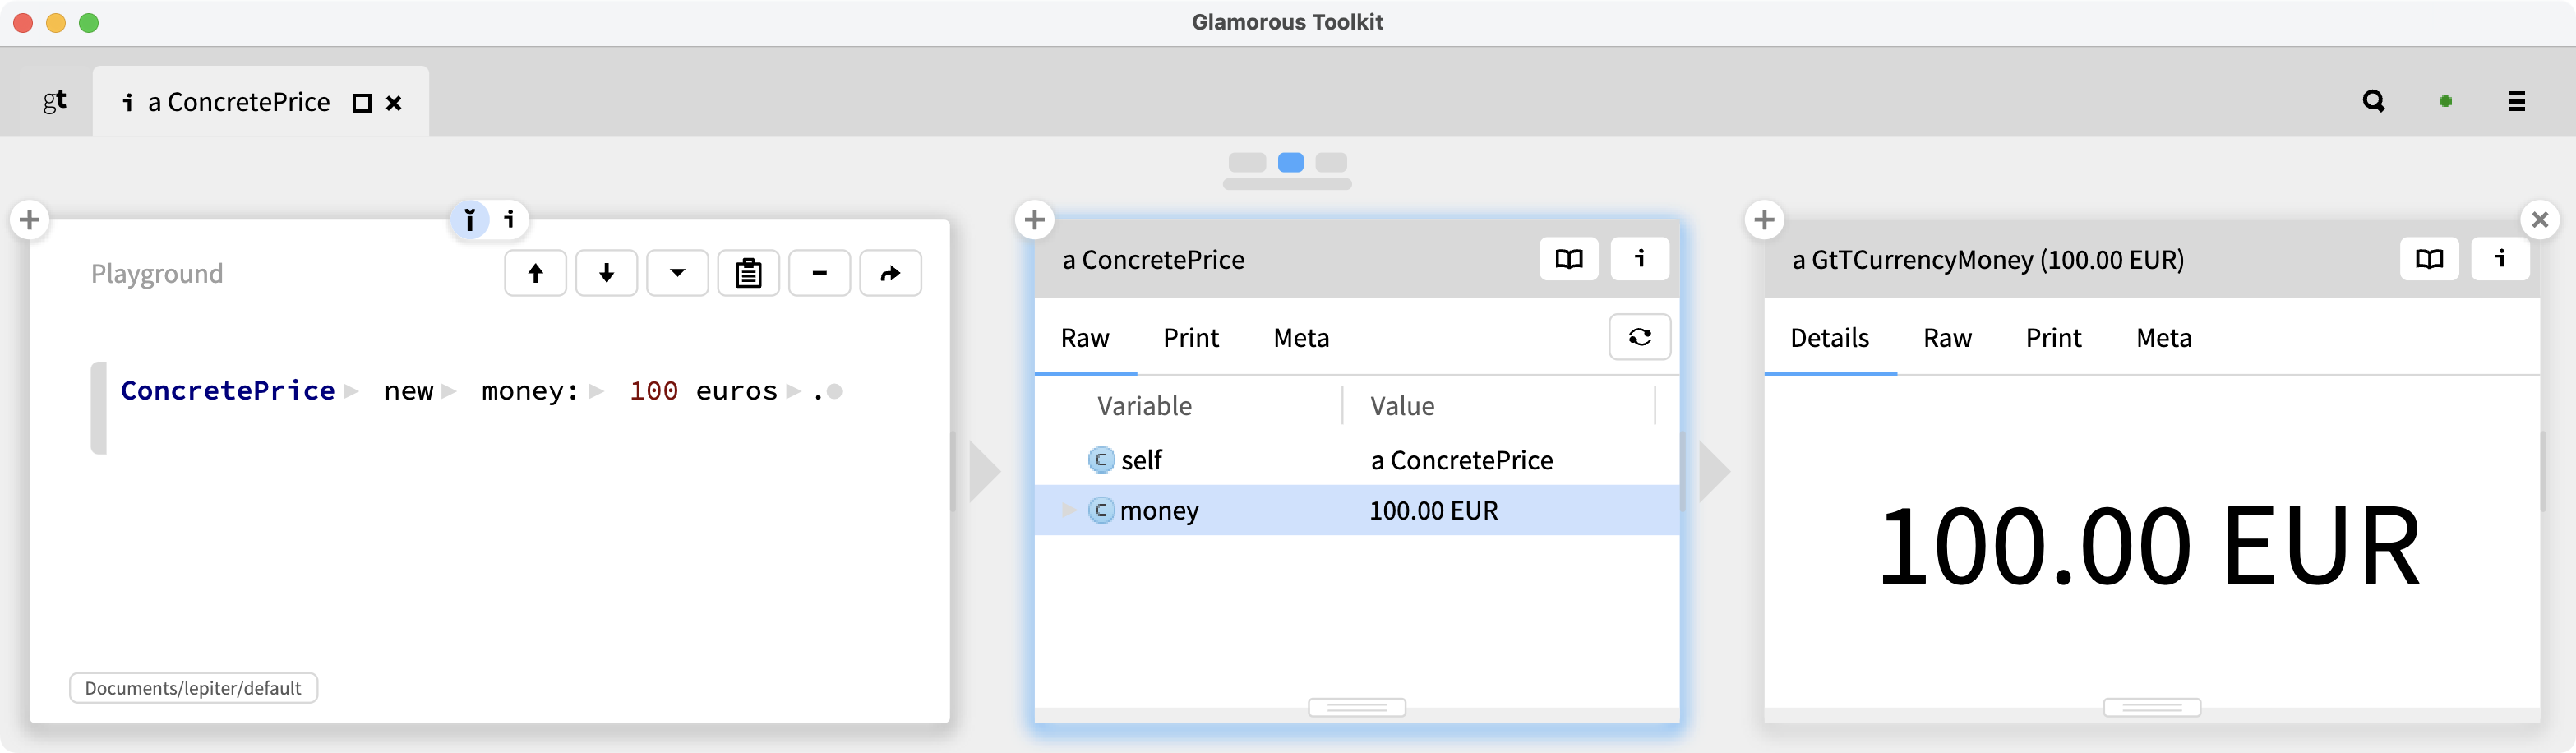
\includegraphics[width=\columnwidth]{edd1-ConcretePrice100Euros}
	\caption{Prototyping a raw Price object.}
  \label{fig:exampleCreationA}
\end{figure}

With the help of \emph{fixit dialogues} (not shown) we create the new class with a \st{money} slot (instance variable) and setter method.
We can then inspect the new, raw \st{ConcretePrice} (middle pane), showing that its \st{money} slot is properly initialized.
We can also inspect the slot's value (rightmost pane).

At this point we realize that it would be nice to have a factory method to create a \st{Price} from a \st{Money} instance.
In the context of the live \st{100 euro} \st{Money} object (\autoref{fig:exampleCreationB} bottom of left pane) we prototype the code to create a price from this instance, namely:
\begin{code}
ConcretePrice new money: self; yourself.
\end{code}

\begin{figure}[h]
  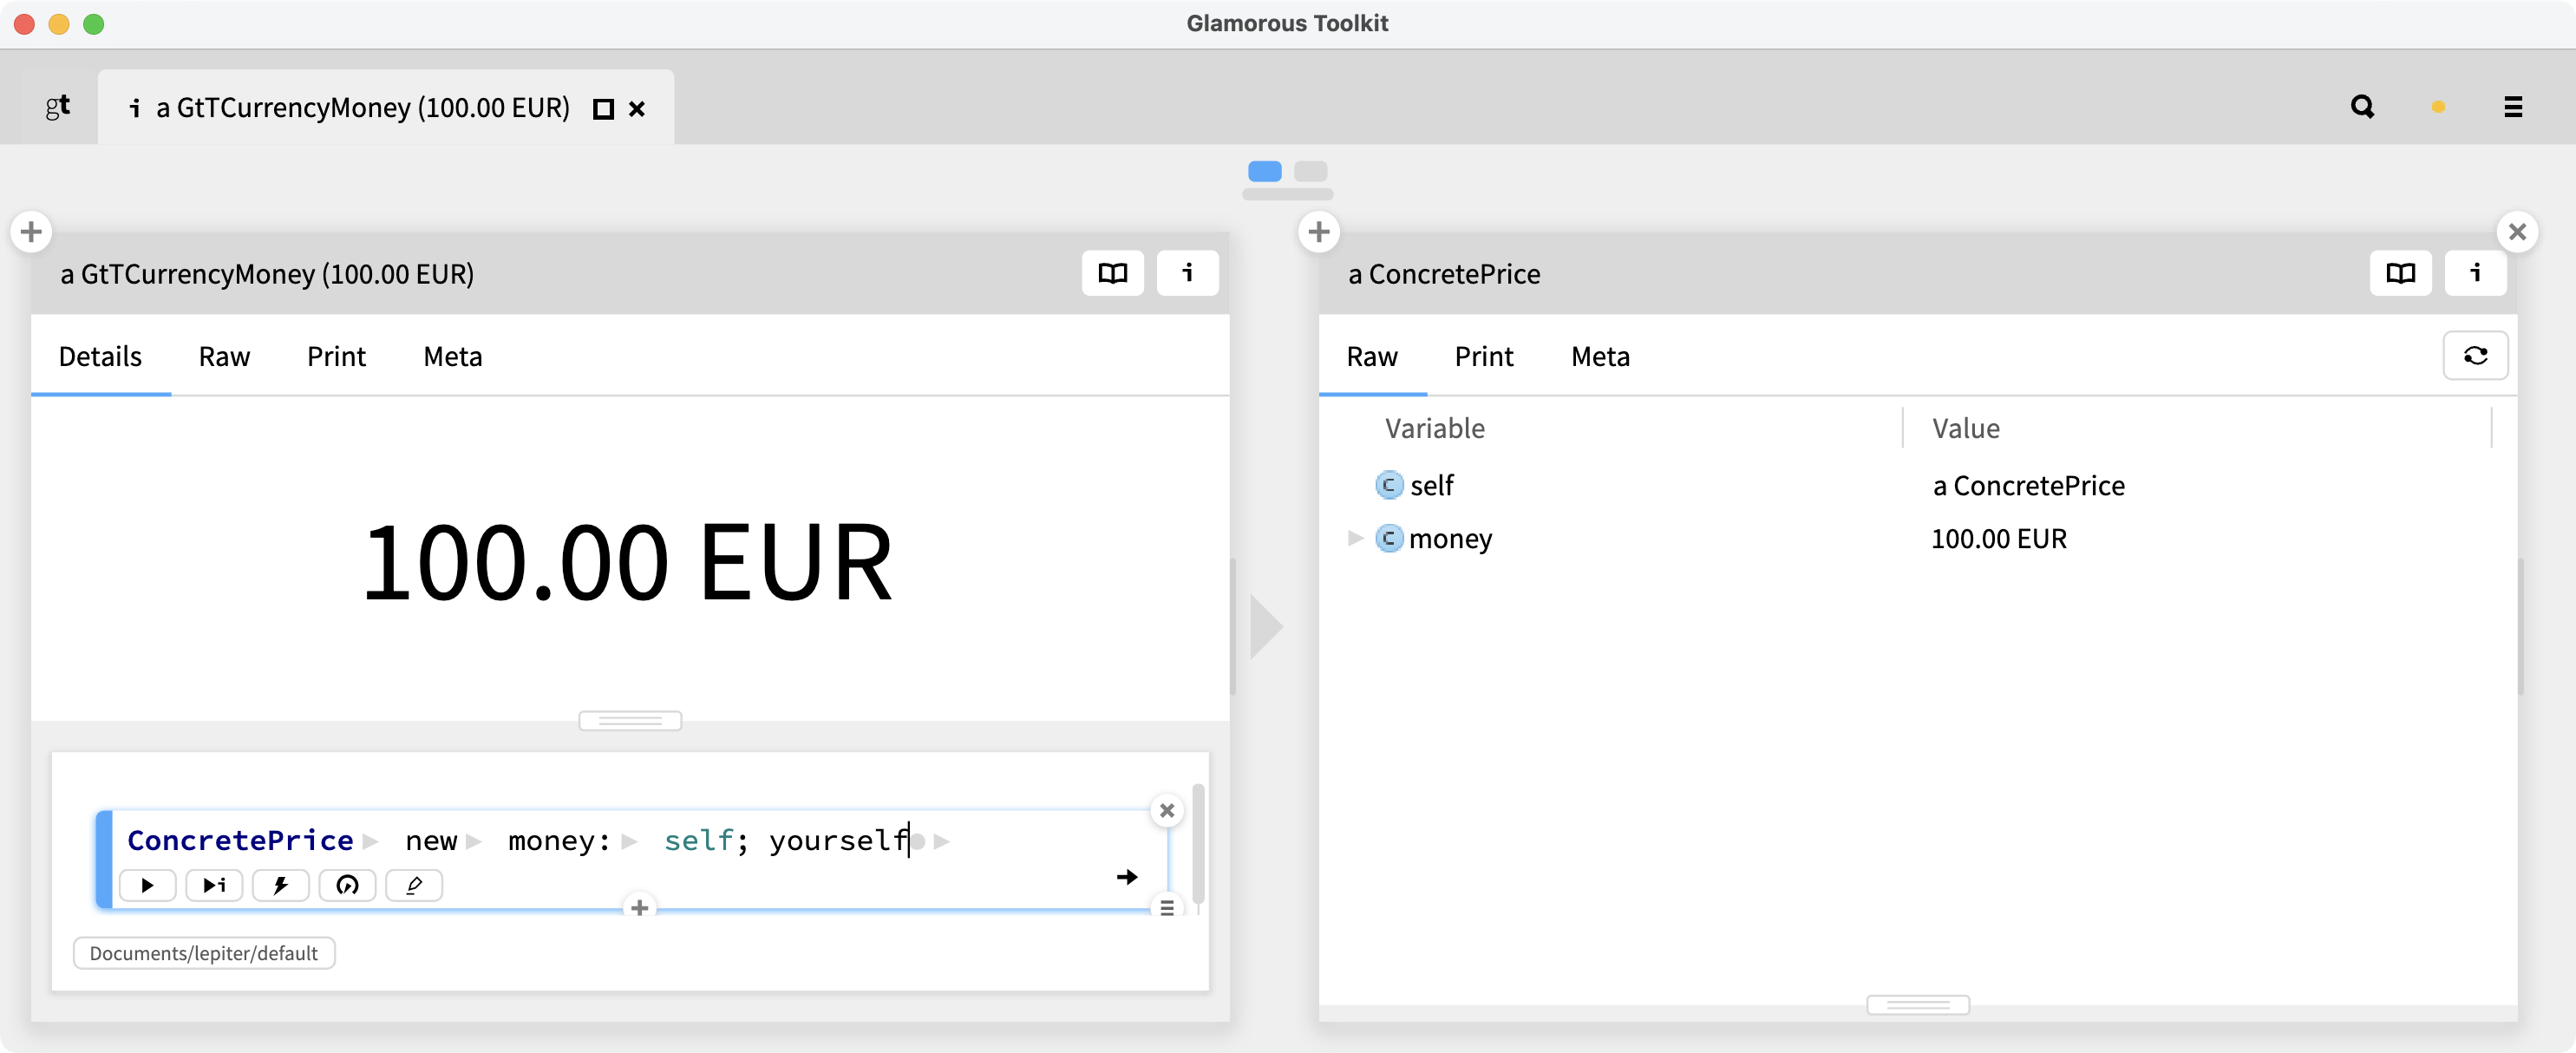
\includegraphics[width=\columnwidth]{edd2-PrototypingAsPrice}
	\caption{Prototyping a factory method.}
  \label{fig:exampleCreationB}
\end{figure}

Note that \st{self} is bound to the live object we are inspecting.
Evaluating this snippet and inspecting the result (right pane) gives us the \st{ConcretePrice} object that we expect.

Now that we have prototyped the factory code, we can extract it as an extension method of the \st{Money} class called \st{asPrice} using an \emph{Extract method} refactoring.
We see the refactored code (\autoref{fig:exampleCreationC}, left pane) as a ``code bubble''~\cite{Brag10a} by expanding \st{asPrice}.
We also see that the refactored snippet still yields the result we want (right pane).

\begin{figure}[h]
  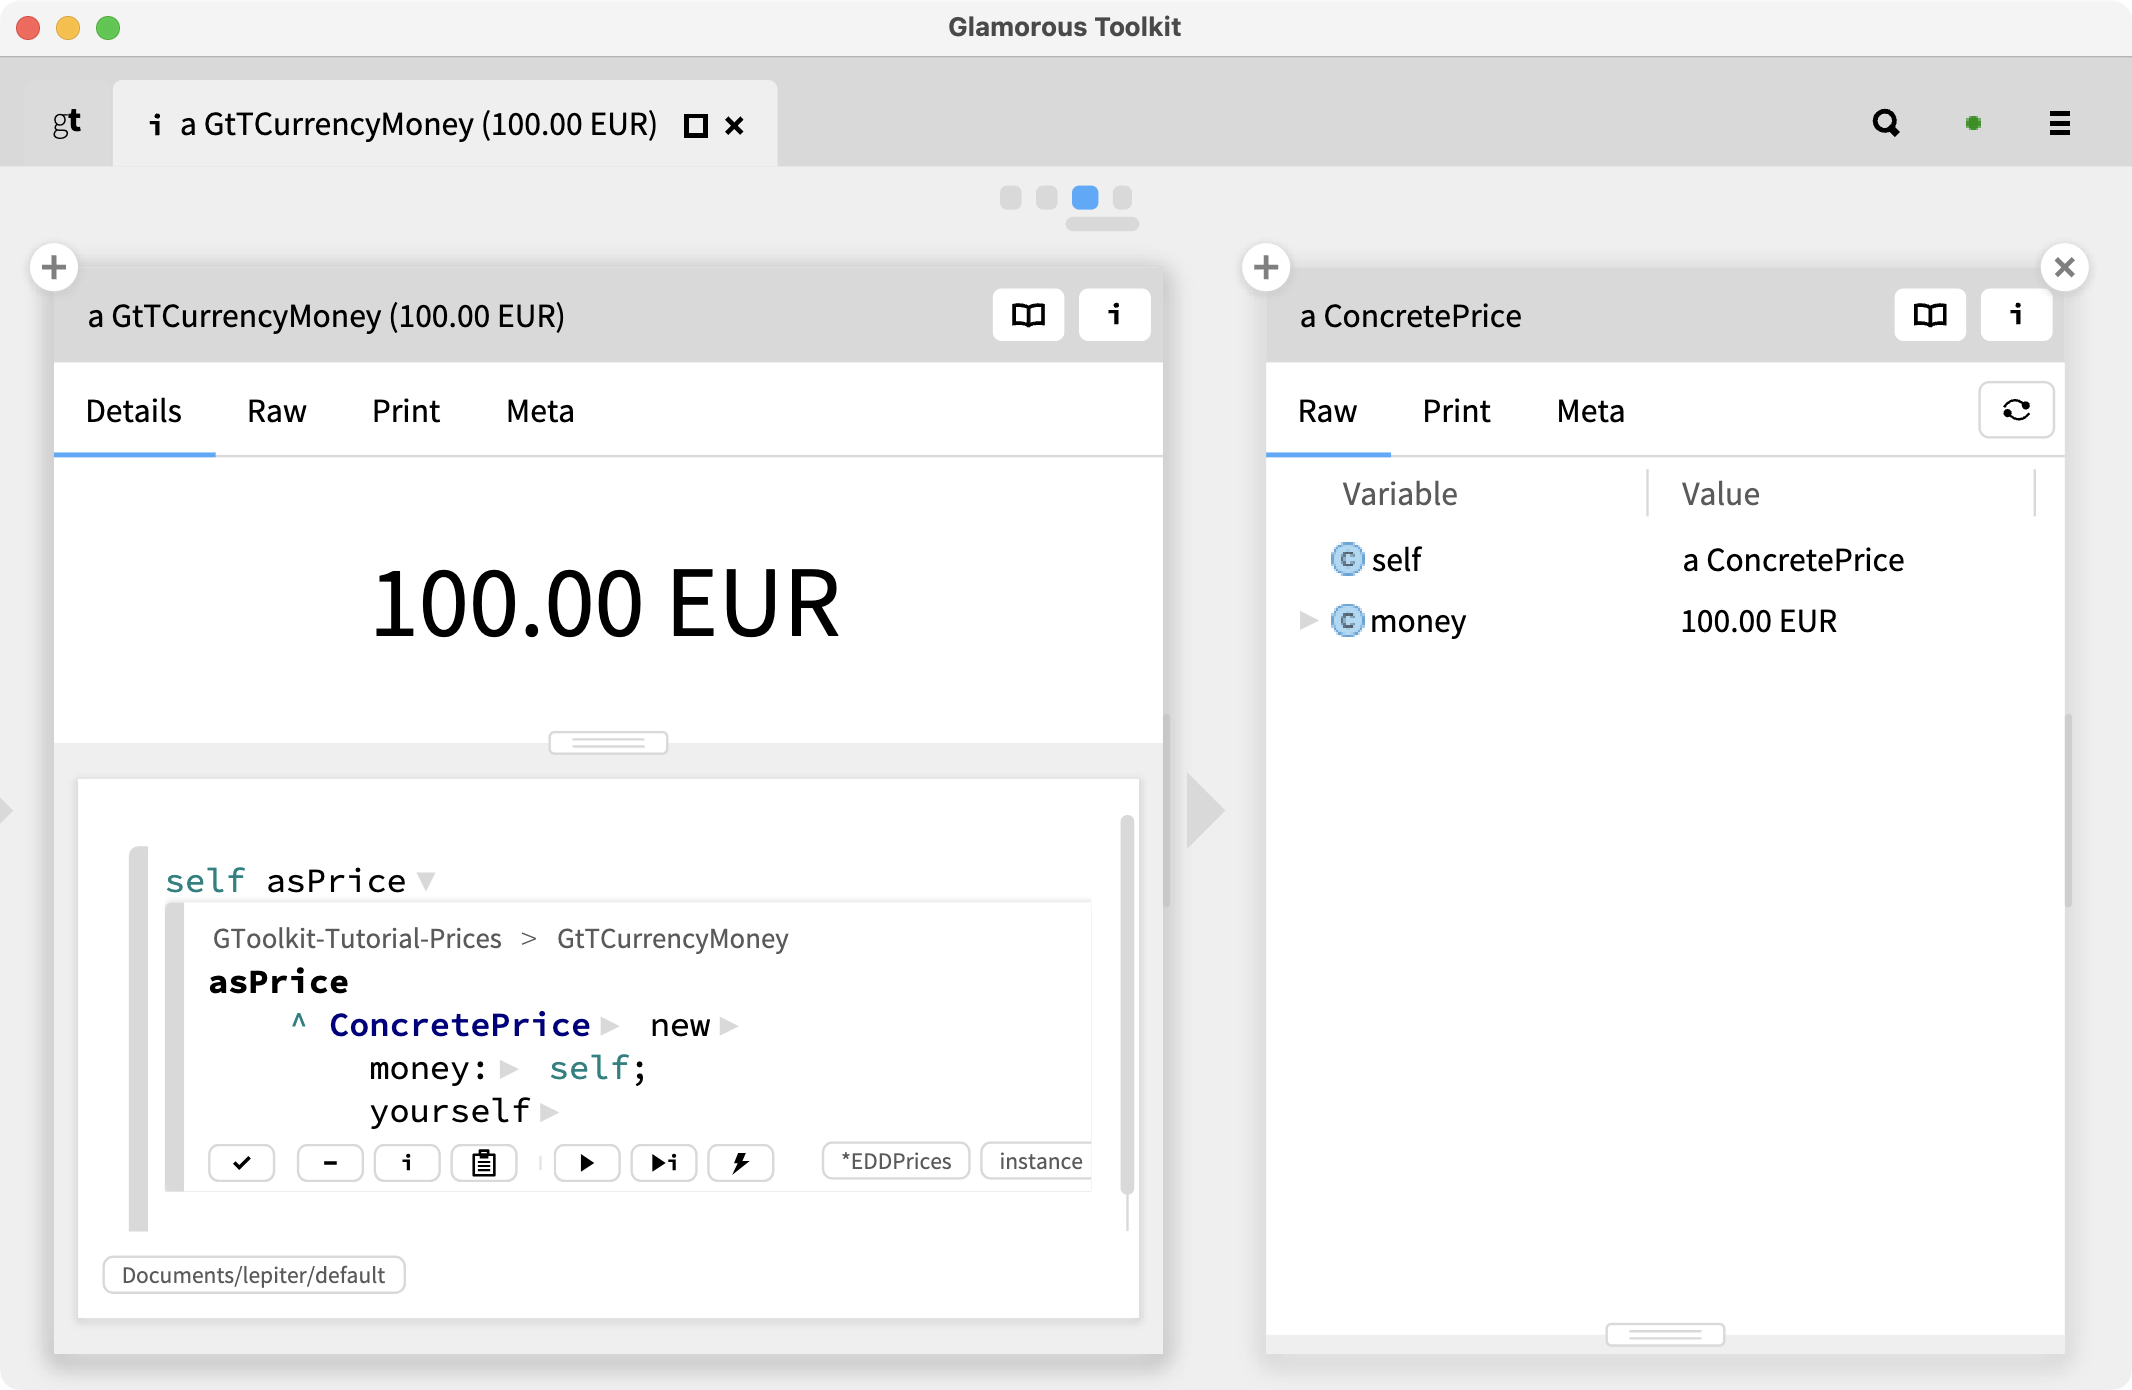
\includegraphics[width=\columnwidth]{edd3-ExtractAsPrice}
	\caption{Extracting a factory method.}
  \label{fig:exampleCreationC}
\end{figure}

Now we can go back to our original snippet (\autoref{fig:exampleCreationD}, left pane) and rewrite it as:
\begin{code}
100 euros asPrice.
\end{code}

\begin{figure}[h]
  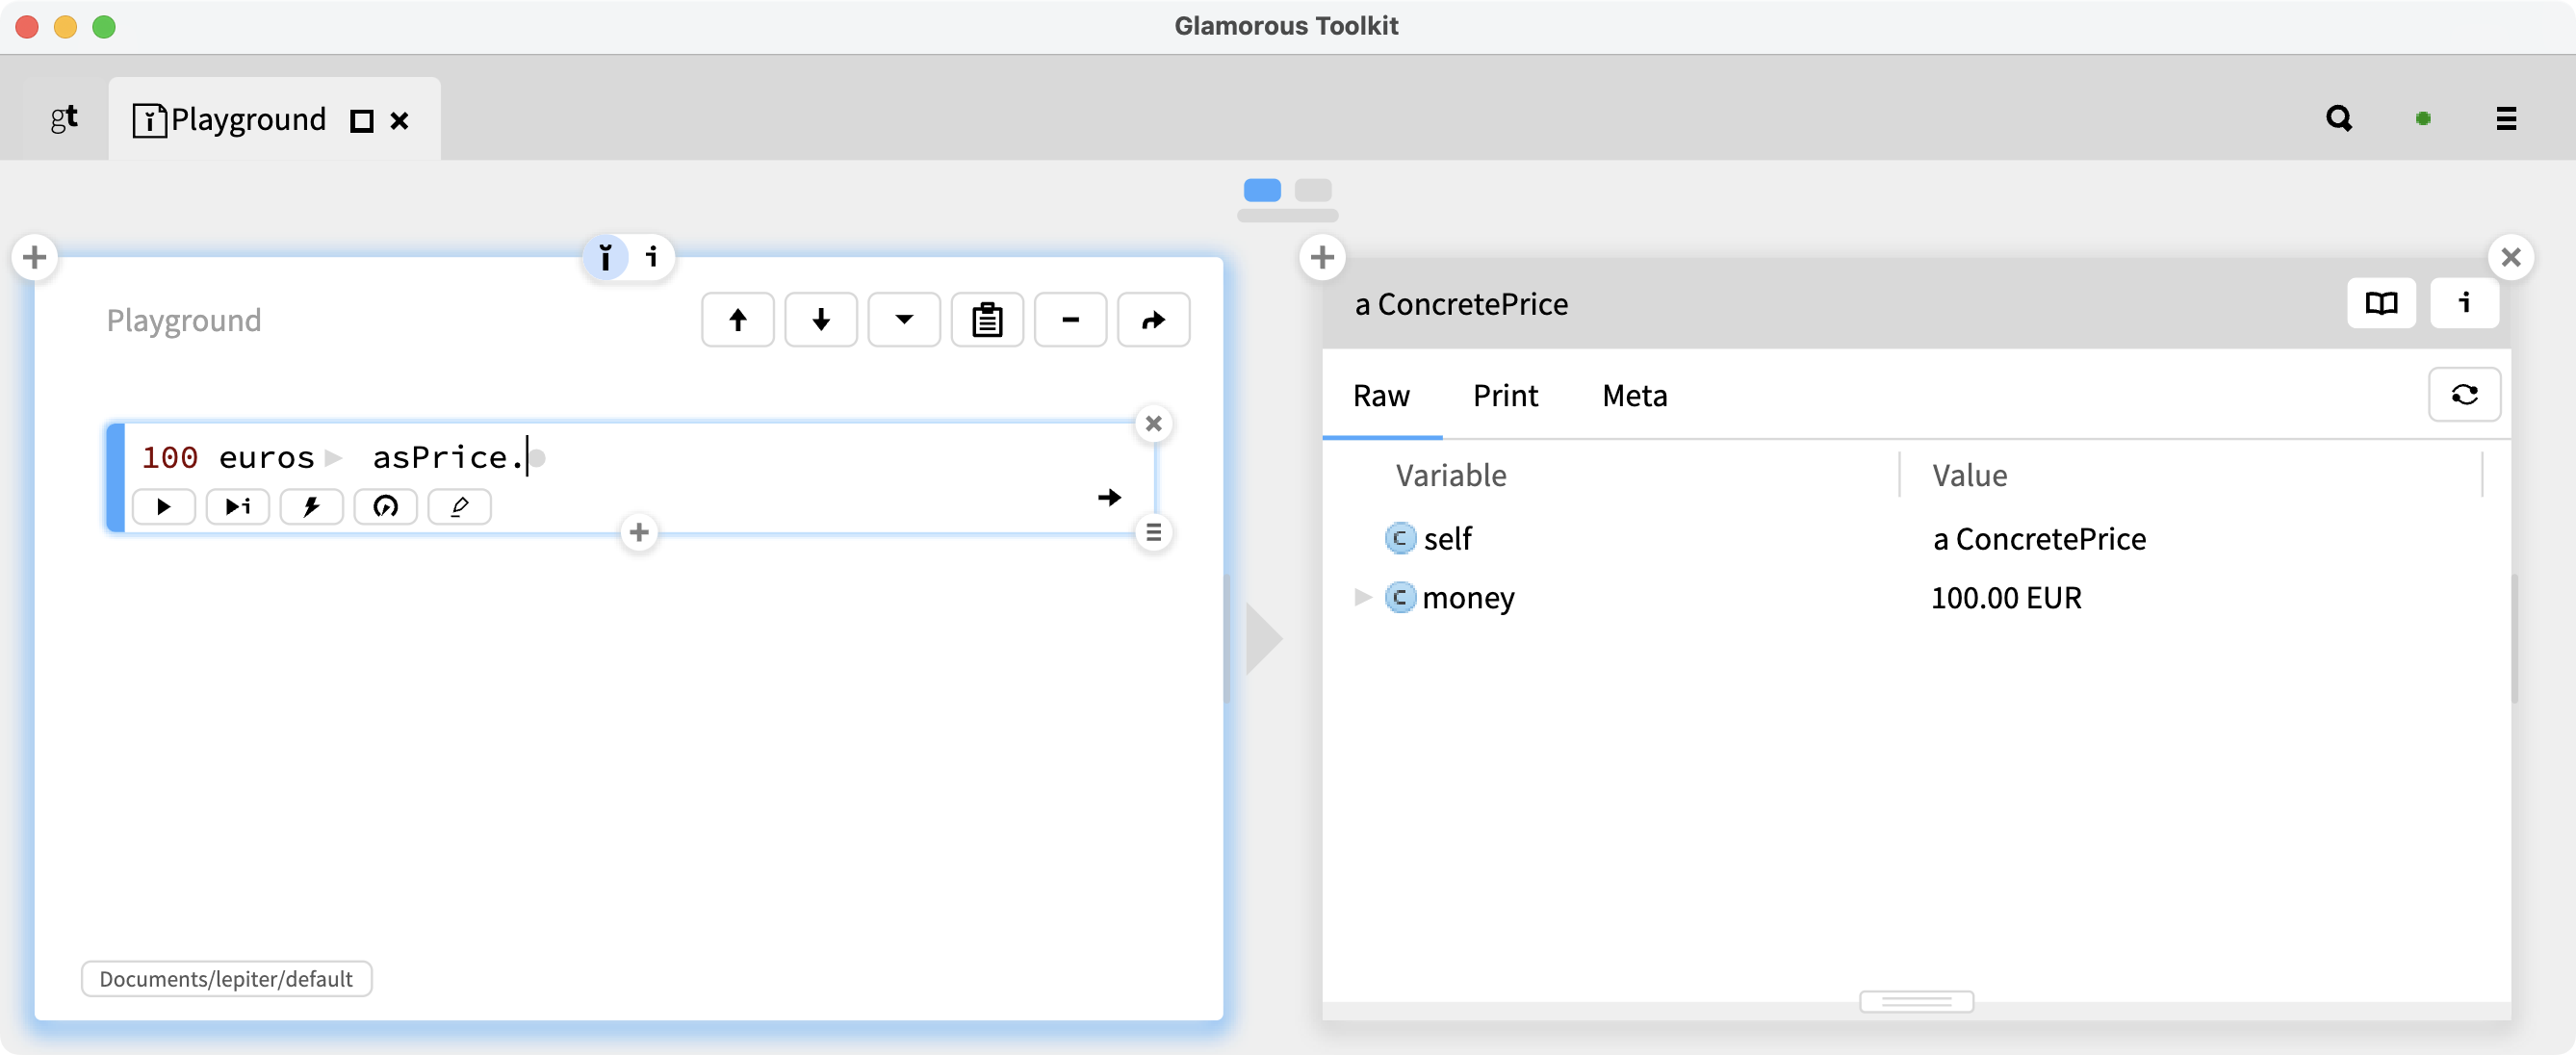
\includegraphics[width=\columnwidth]{edd4-MoneyAsPrice}
	\caption{Rewriting the initial snippet.}
  \label{fig:exampleCreationD}
\end{figure}

Now we have a nice snippet that creates an example that interests us.
In \autoref{fig:exampleExtractionA} we apply an \emph{Extract example} refactoring to create a new \st{PriceExamples} class with a \st{hundredEuros} example  method.
It is simply a method with a \st{<gtExample>} annotation (analogous to Java method annotations) that flags it as an example method, and which returns the object of interest (\autoref{fig:exampleExtractionB}, left pane with code bubble).
Our example method still does not test anything, so let's prototype that too.
We would expect our \st{hundredEuros} example to be equal to another instance that is created in the same way.

\begin{figure}[h]
  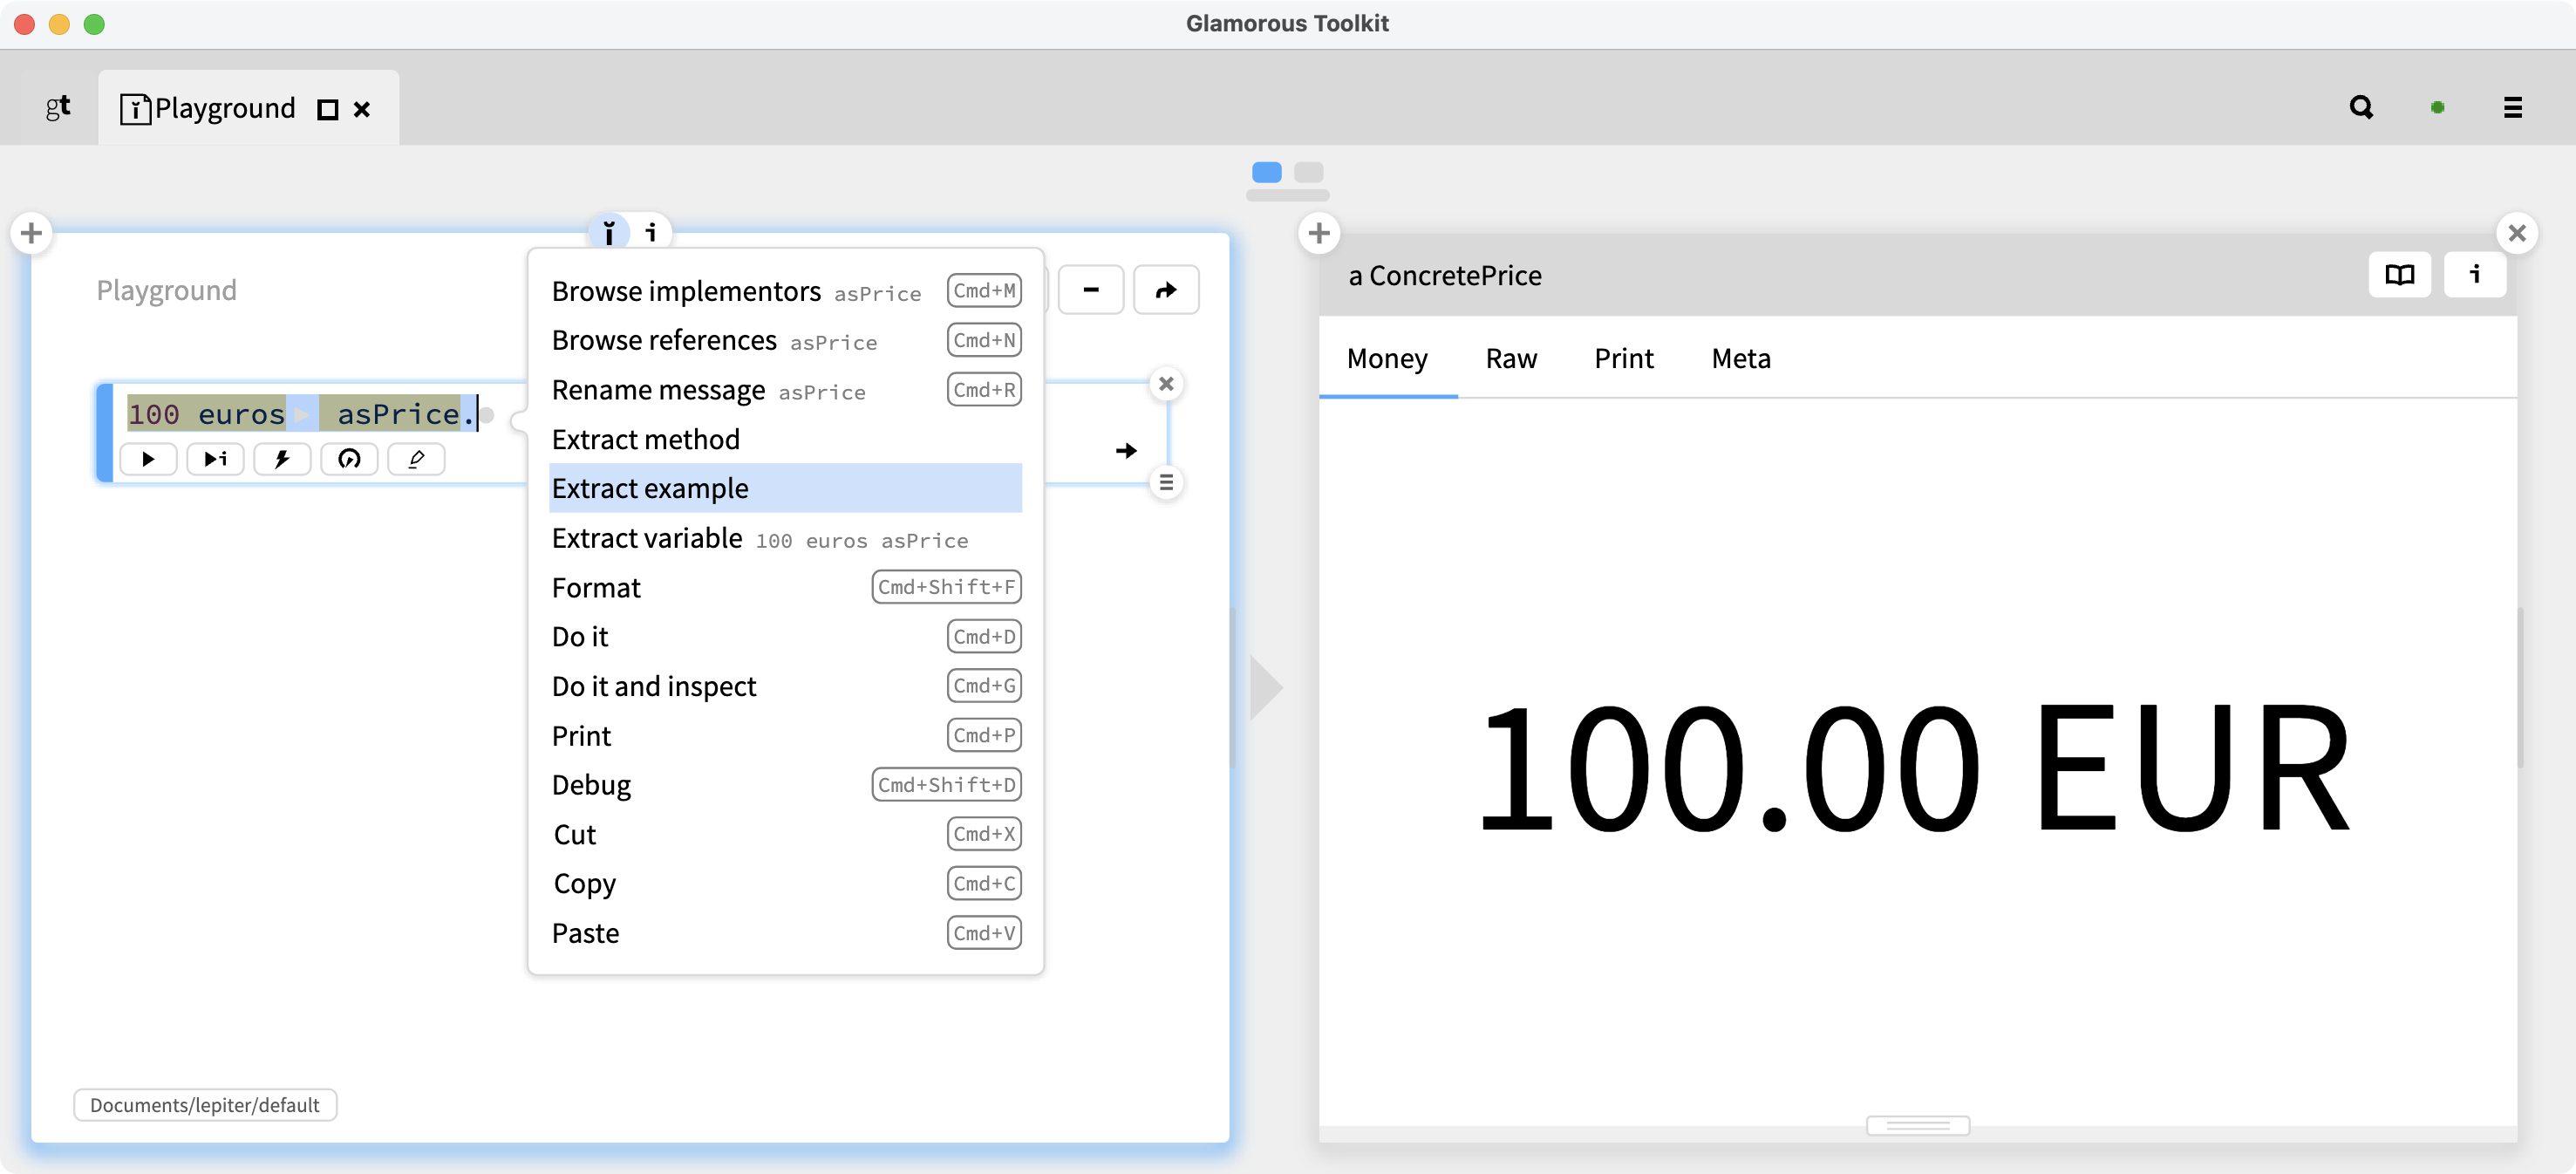
\includegraphics[width=\columnwidth]{edd5-ExtractingExample}
	\caption{Extracting an example method.}
  \label{fig:exampleExtractionA}
\end{figure}

\begin{figure}[h]
  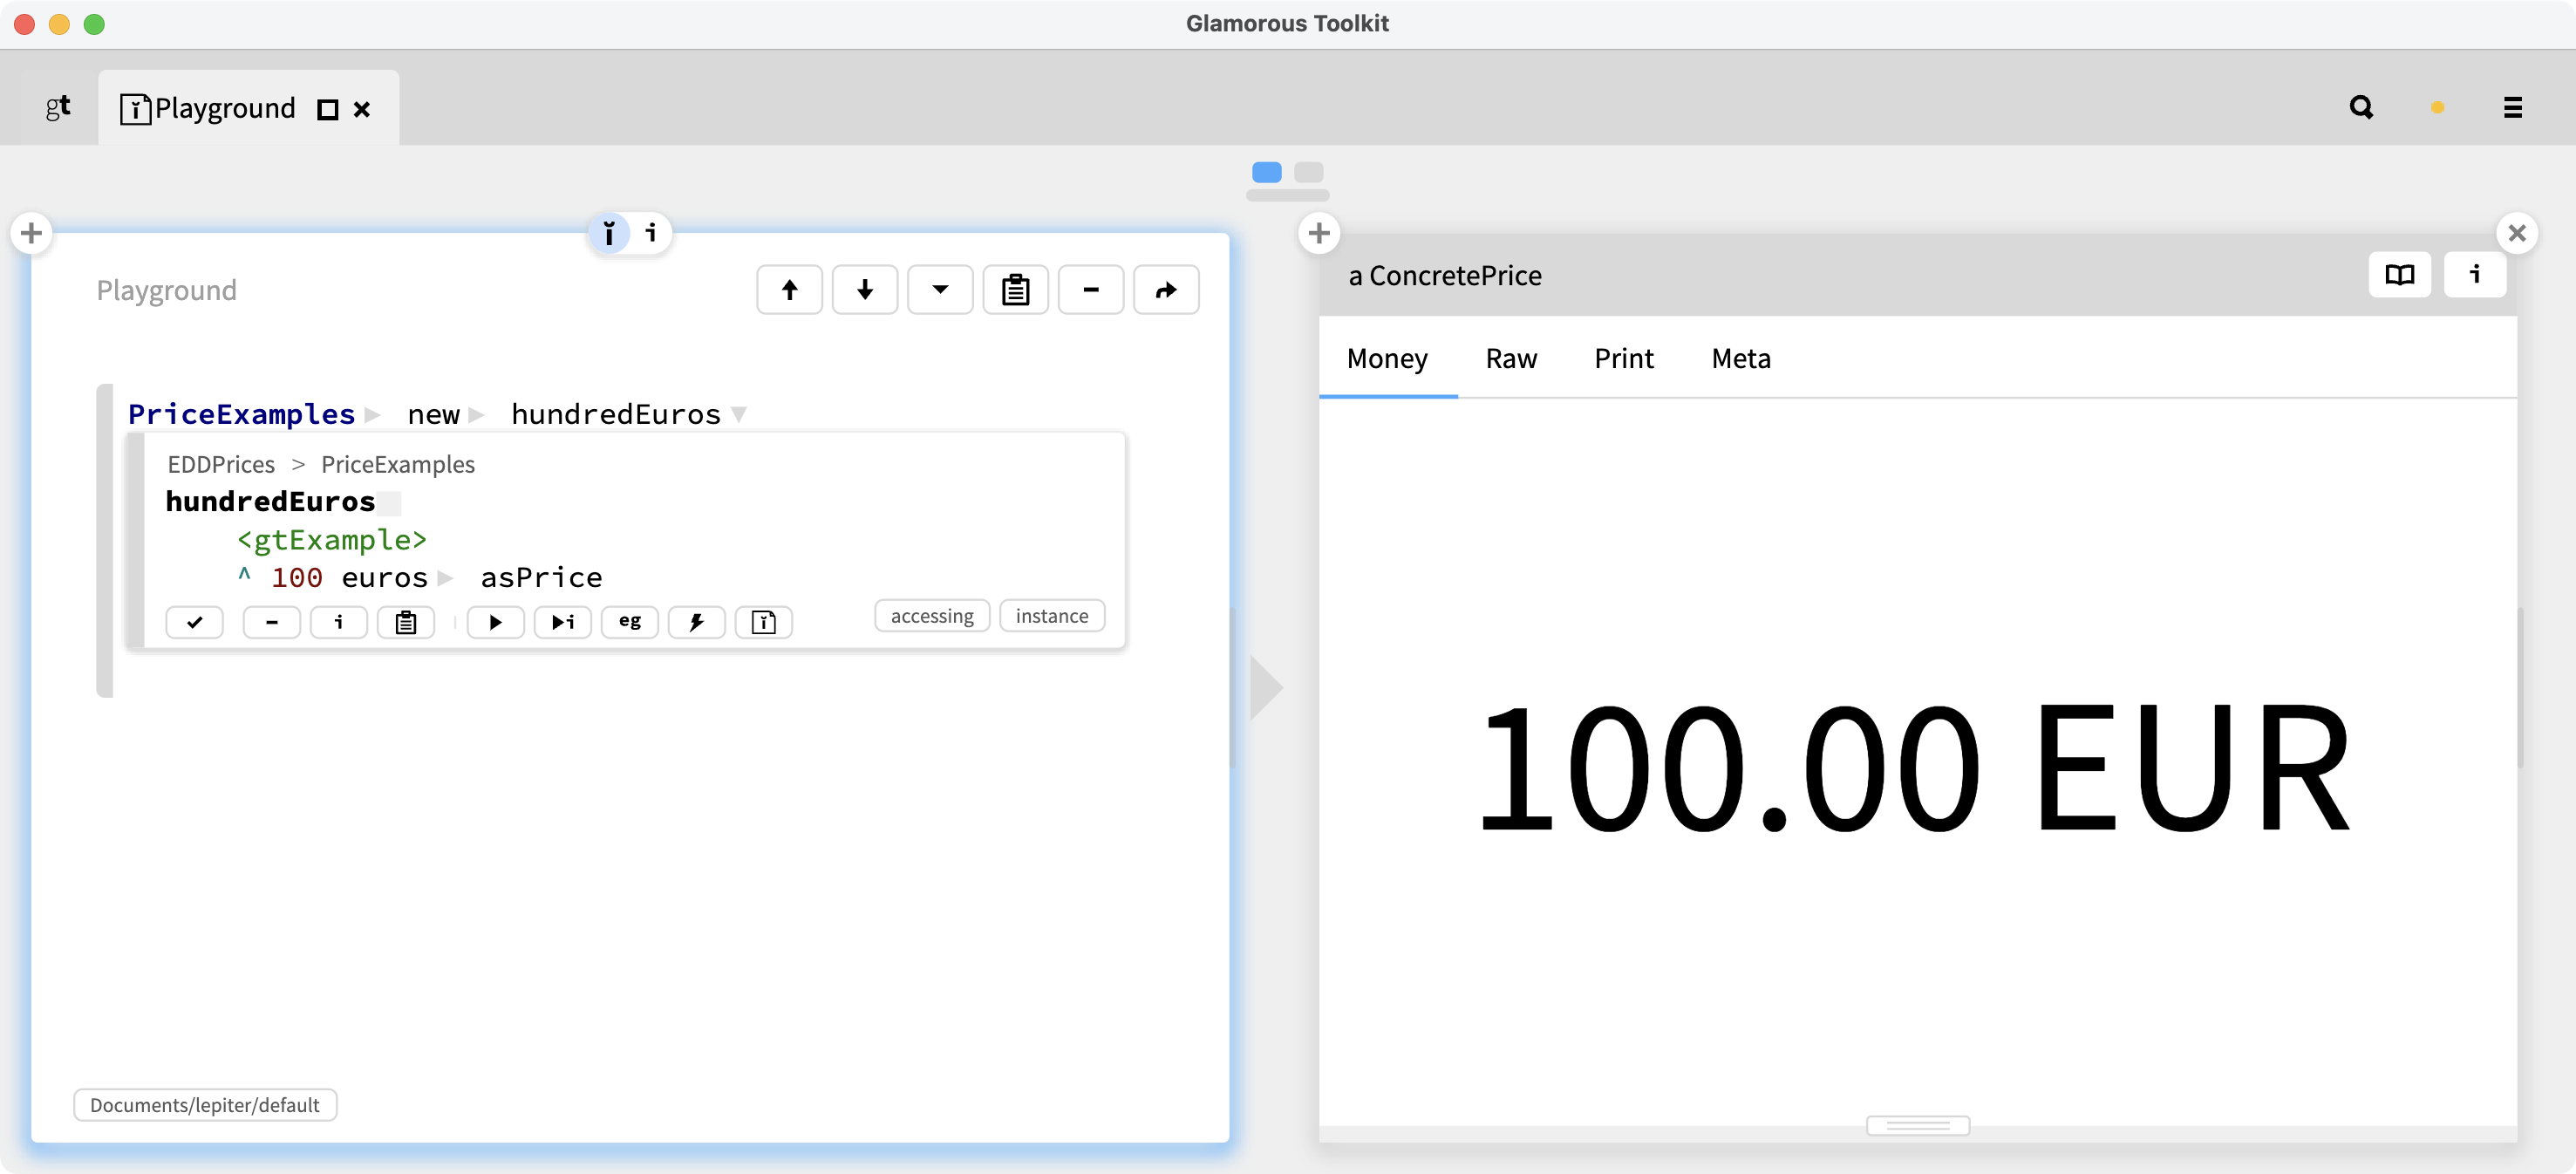
\includegraphics[width=\columnwidth]{edd6-PriceExample}
	\caption{The extracted example method.}
  \label{fig:exampleExtractionB}
\end{figure}

Within the context of the live example (\autoref{fig:exampleExtractionC}, left pane) we prototype the assertion that this example object (\ie \st{self}) is equal to another object created the same way.
Unfortunately this fails (right pane) because our new \st{ConcretePrice} object has not implemented equality, so equality defaults to object identity.
\begin{figure}[h]
  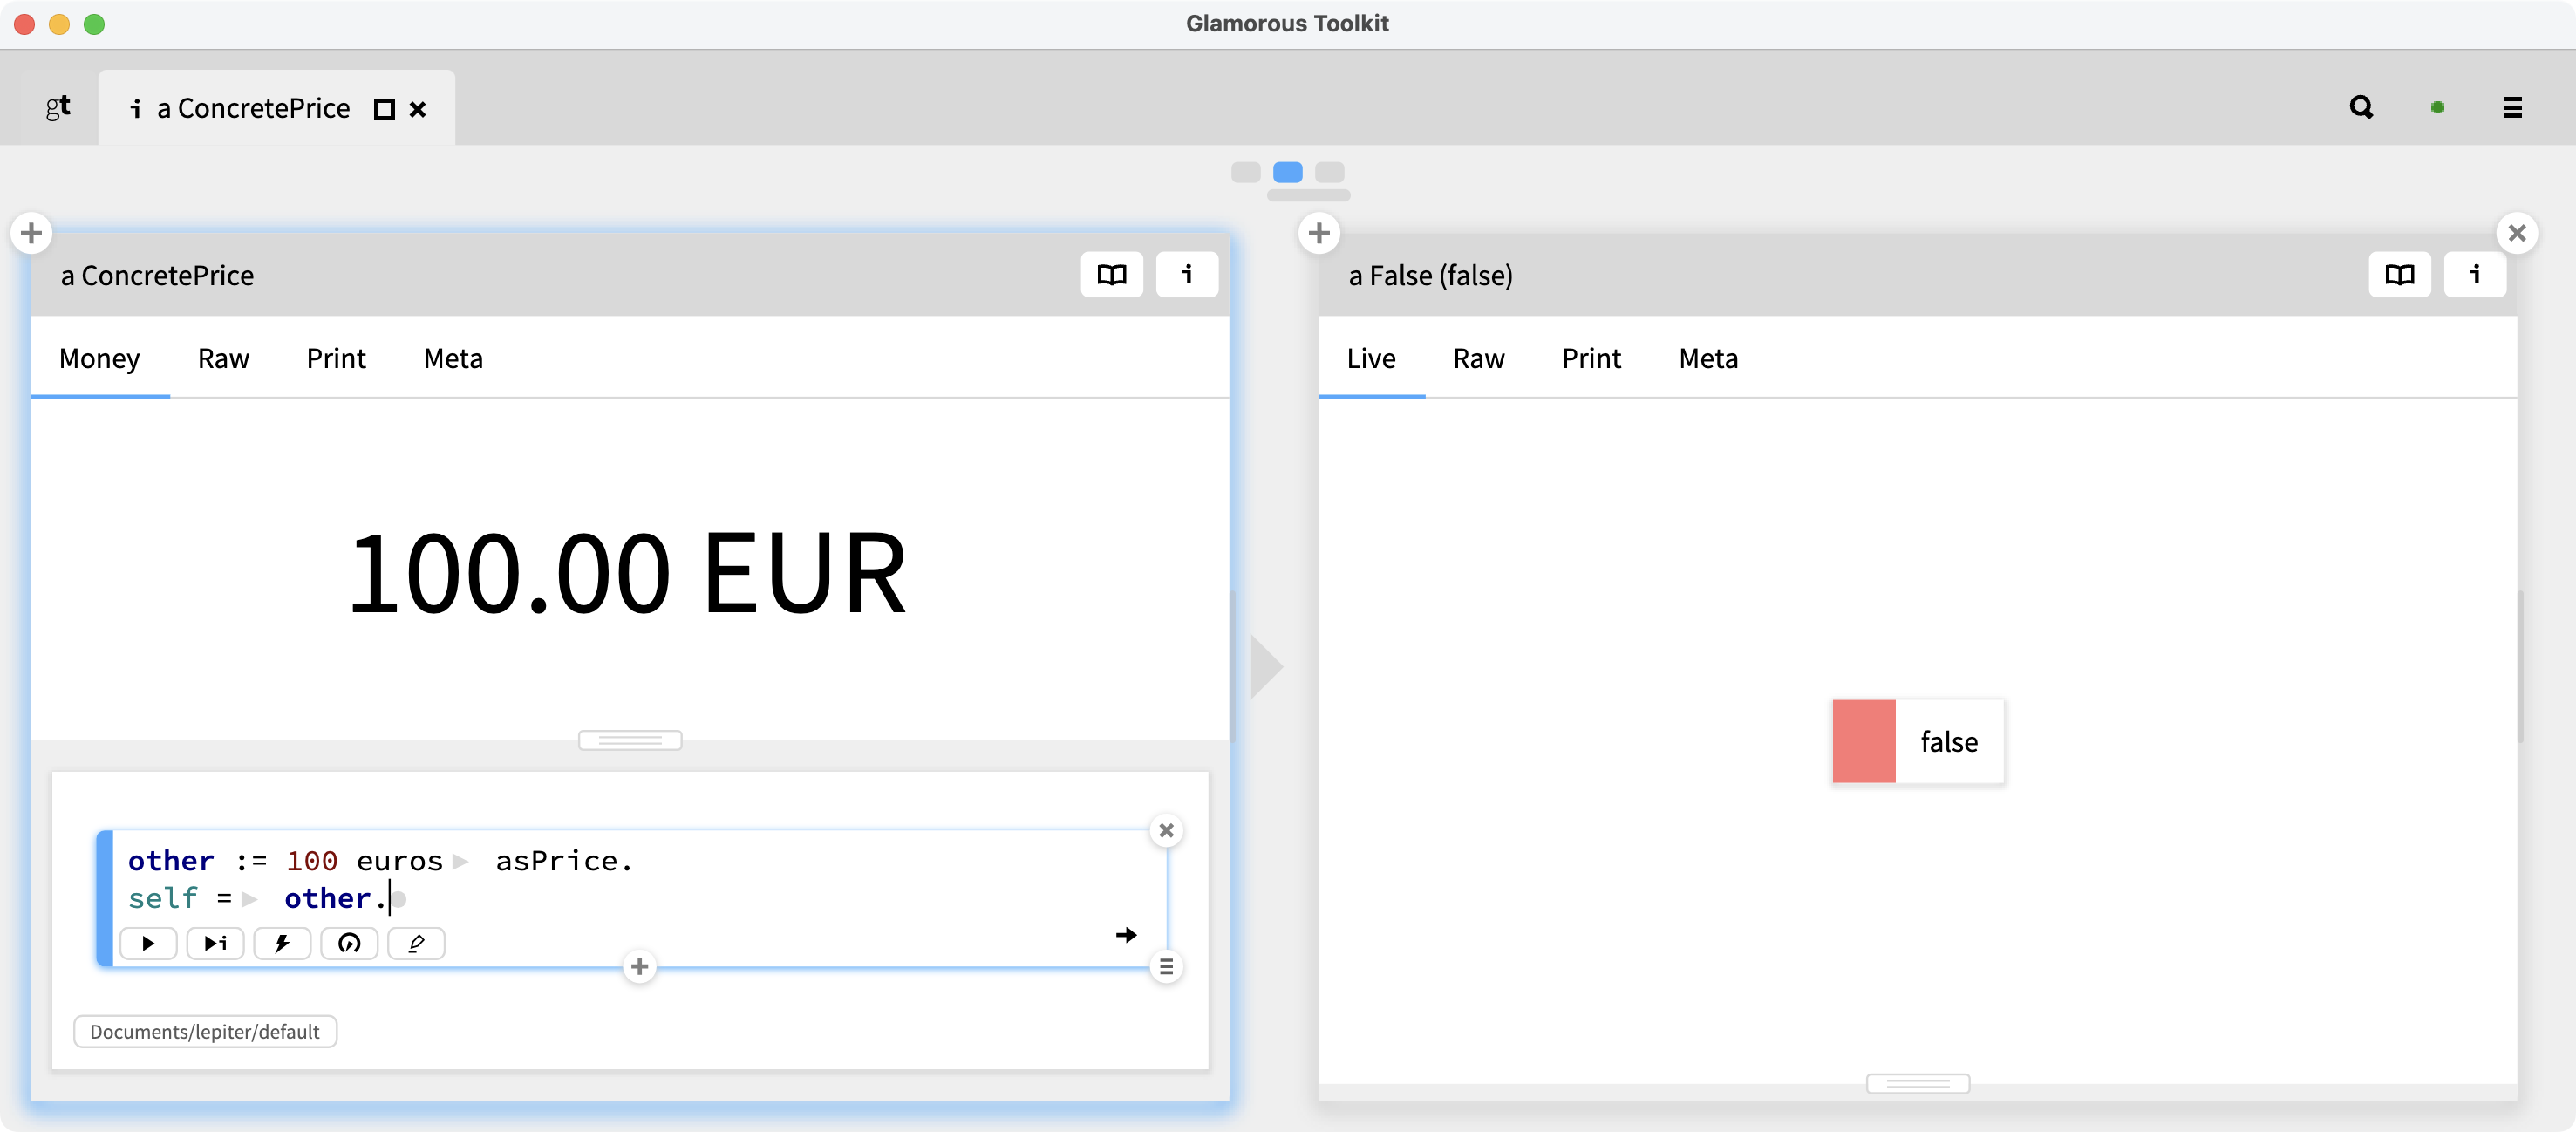
\includegraphics[width=\columnwidth]{edd7-FailedTest}
	\caption{Prototyping an assertion.}
  \label{fig:exampleExtractionC}
\end{figure}

We implement the missing method, and now update our example method (\autoref{fig:exampleExtractionD} left pane) with the new assertion.
If we evaluate this example method, it is not only green (left), but also returns an example we can explore (right).

\begin{figure}[h]
  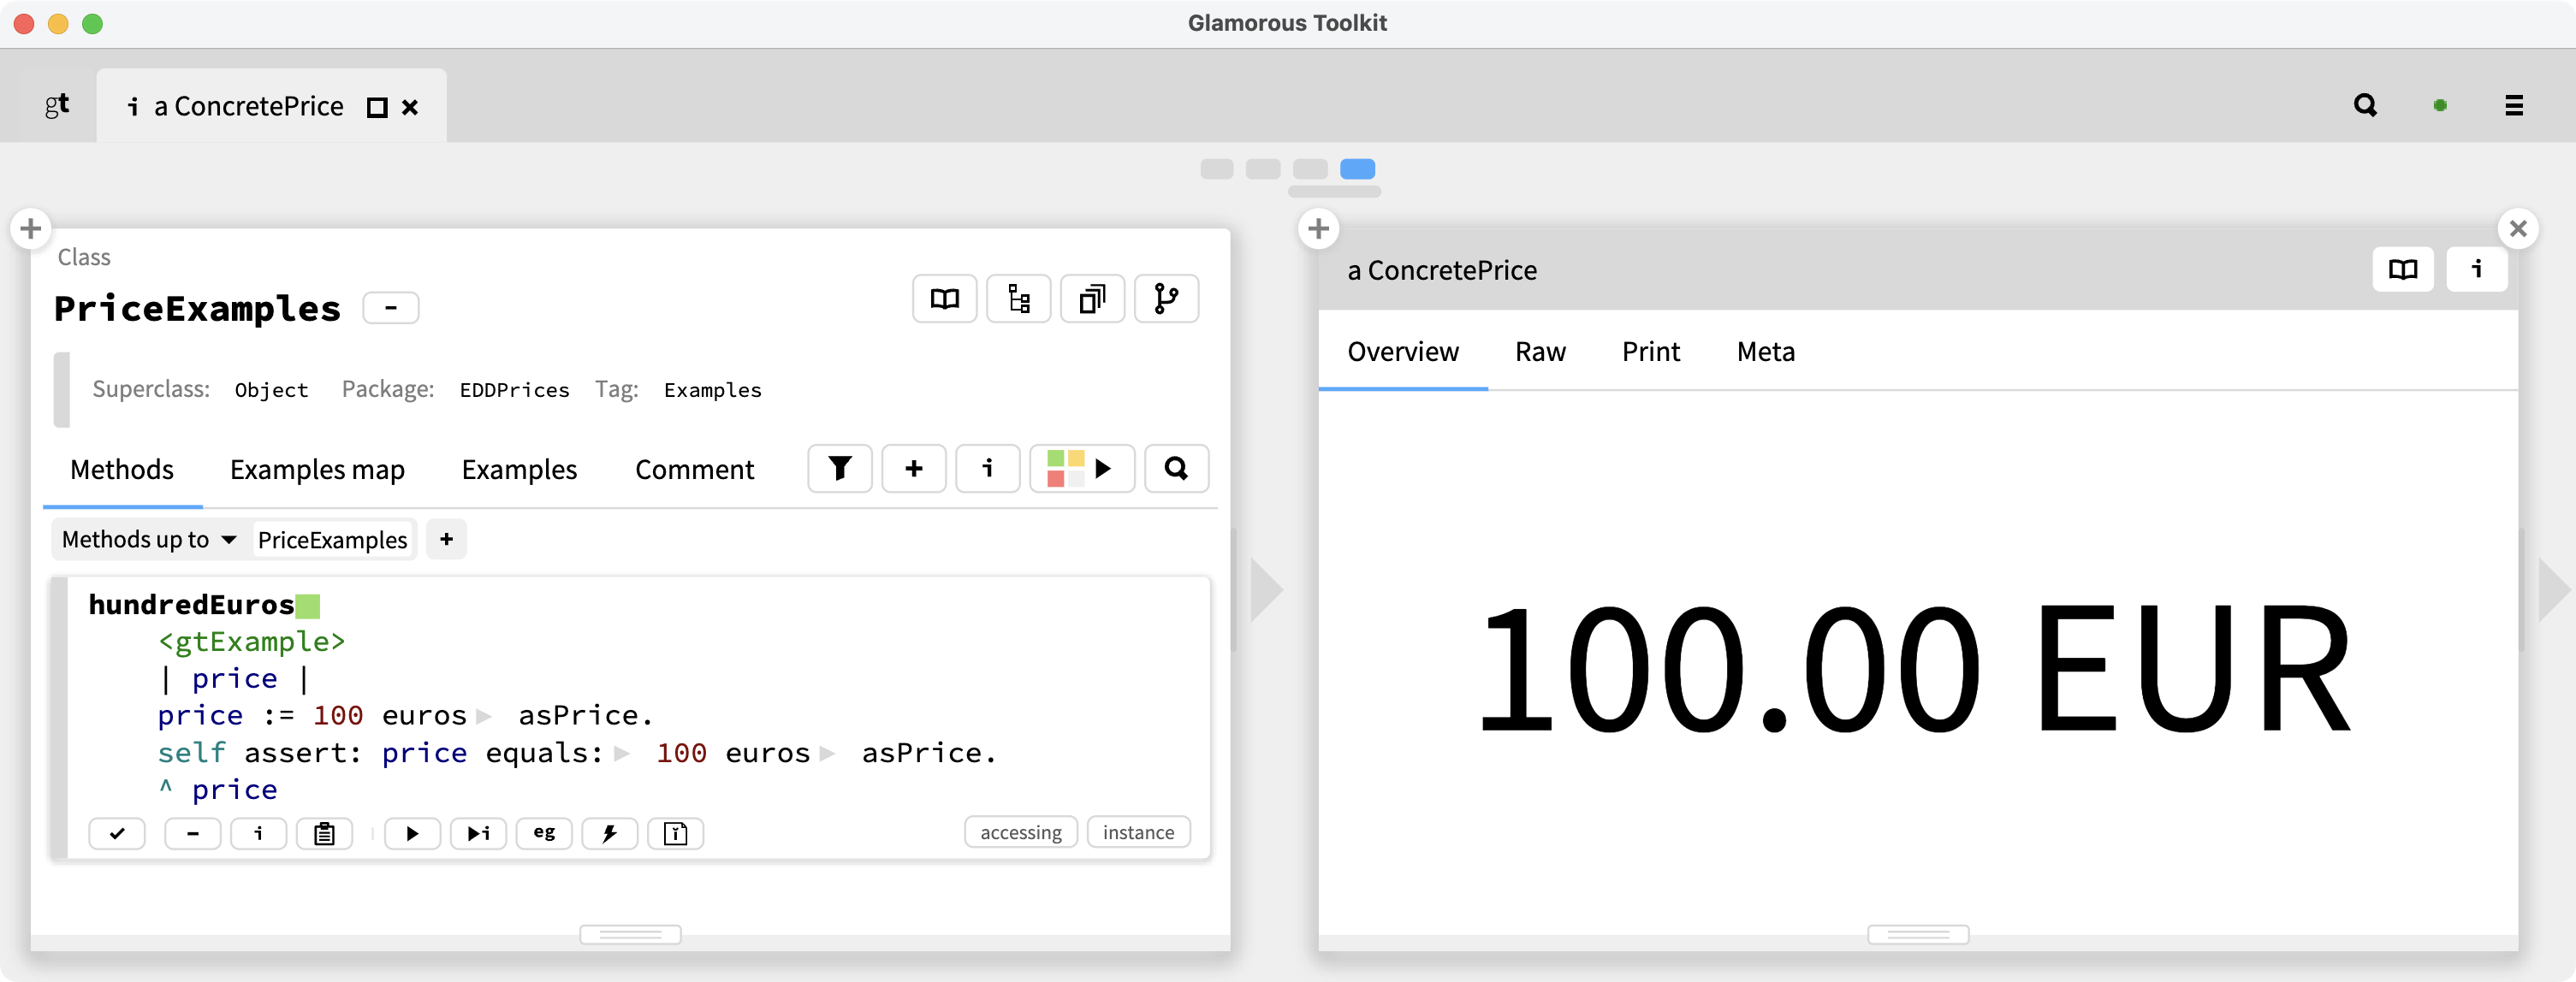
\includegraphics[width=\columnwidth]{edd8-ExampleWithAssertions}
	\caption{Adding the assertion to the example method.}
  \label{fig:exampleExtractionD}
\end{figure}

% ============================================================
\section{Moldable Examples}\label{sec:moldable}

When we inspect our \st{hundredEuro} example (\autoref{fig:exampleExtractionD}), instead of the original ``raw'' inspector view we see a new \emph{Overview} view showing the value of the concrete price.
How did this happen?
Actually there is a step missing that we will now explain.

\emph{Moldable development} is an approach to constructing \emph{explainable software systems} by augmenting the objects of the software system with dozens of tiny analysis tools that can answer questions about the system.
It can be understood as a refinement of EDD in which objects (examples) are enhanced with custom tools during the development process.

Moldable development is made possible with the help of \emph{moldable tools}~\cite{Chis17a}, such as code browsers, debuggers, and object inspectors, that can adapt themselves to the run-time context of an application to enable these analysis tools.
% Chis17a Moldable Tools for Object-oriented Development
For example, consider the screenshot of a Ludo\footnote{\url{https://en.m.wikipedia.org/wiki/Ludo}} game in figure \autoref{fig:ludoViews}.
At the left we see in an object inspector a GUI \emph{Board} view of a running instance of the game that has terminated with player B winning.
In the middle we see a \emph{Moves} view of the same instance, showing us all the past moves leading to the concluding state of the game.
Finally, at the right we inspect a particular move, showing us how the game state was updated in move \#109.

\begin{figure}[h]
  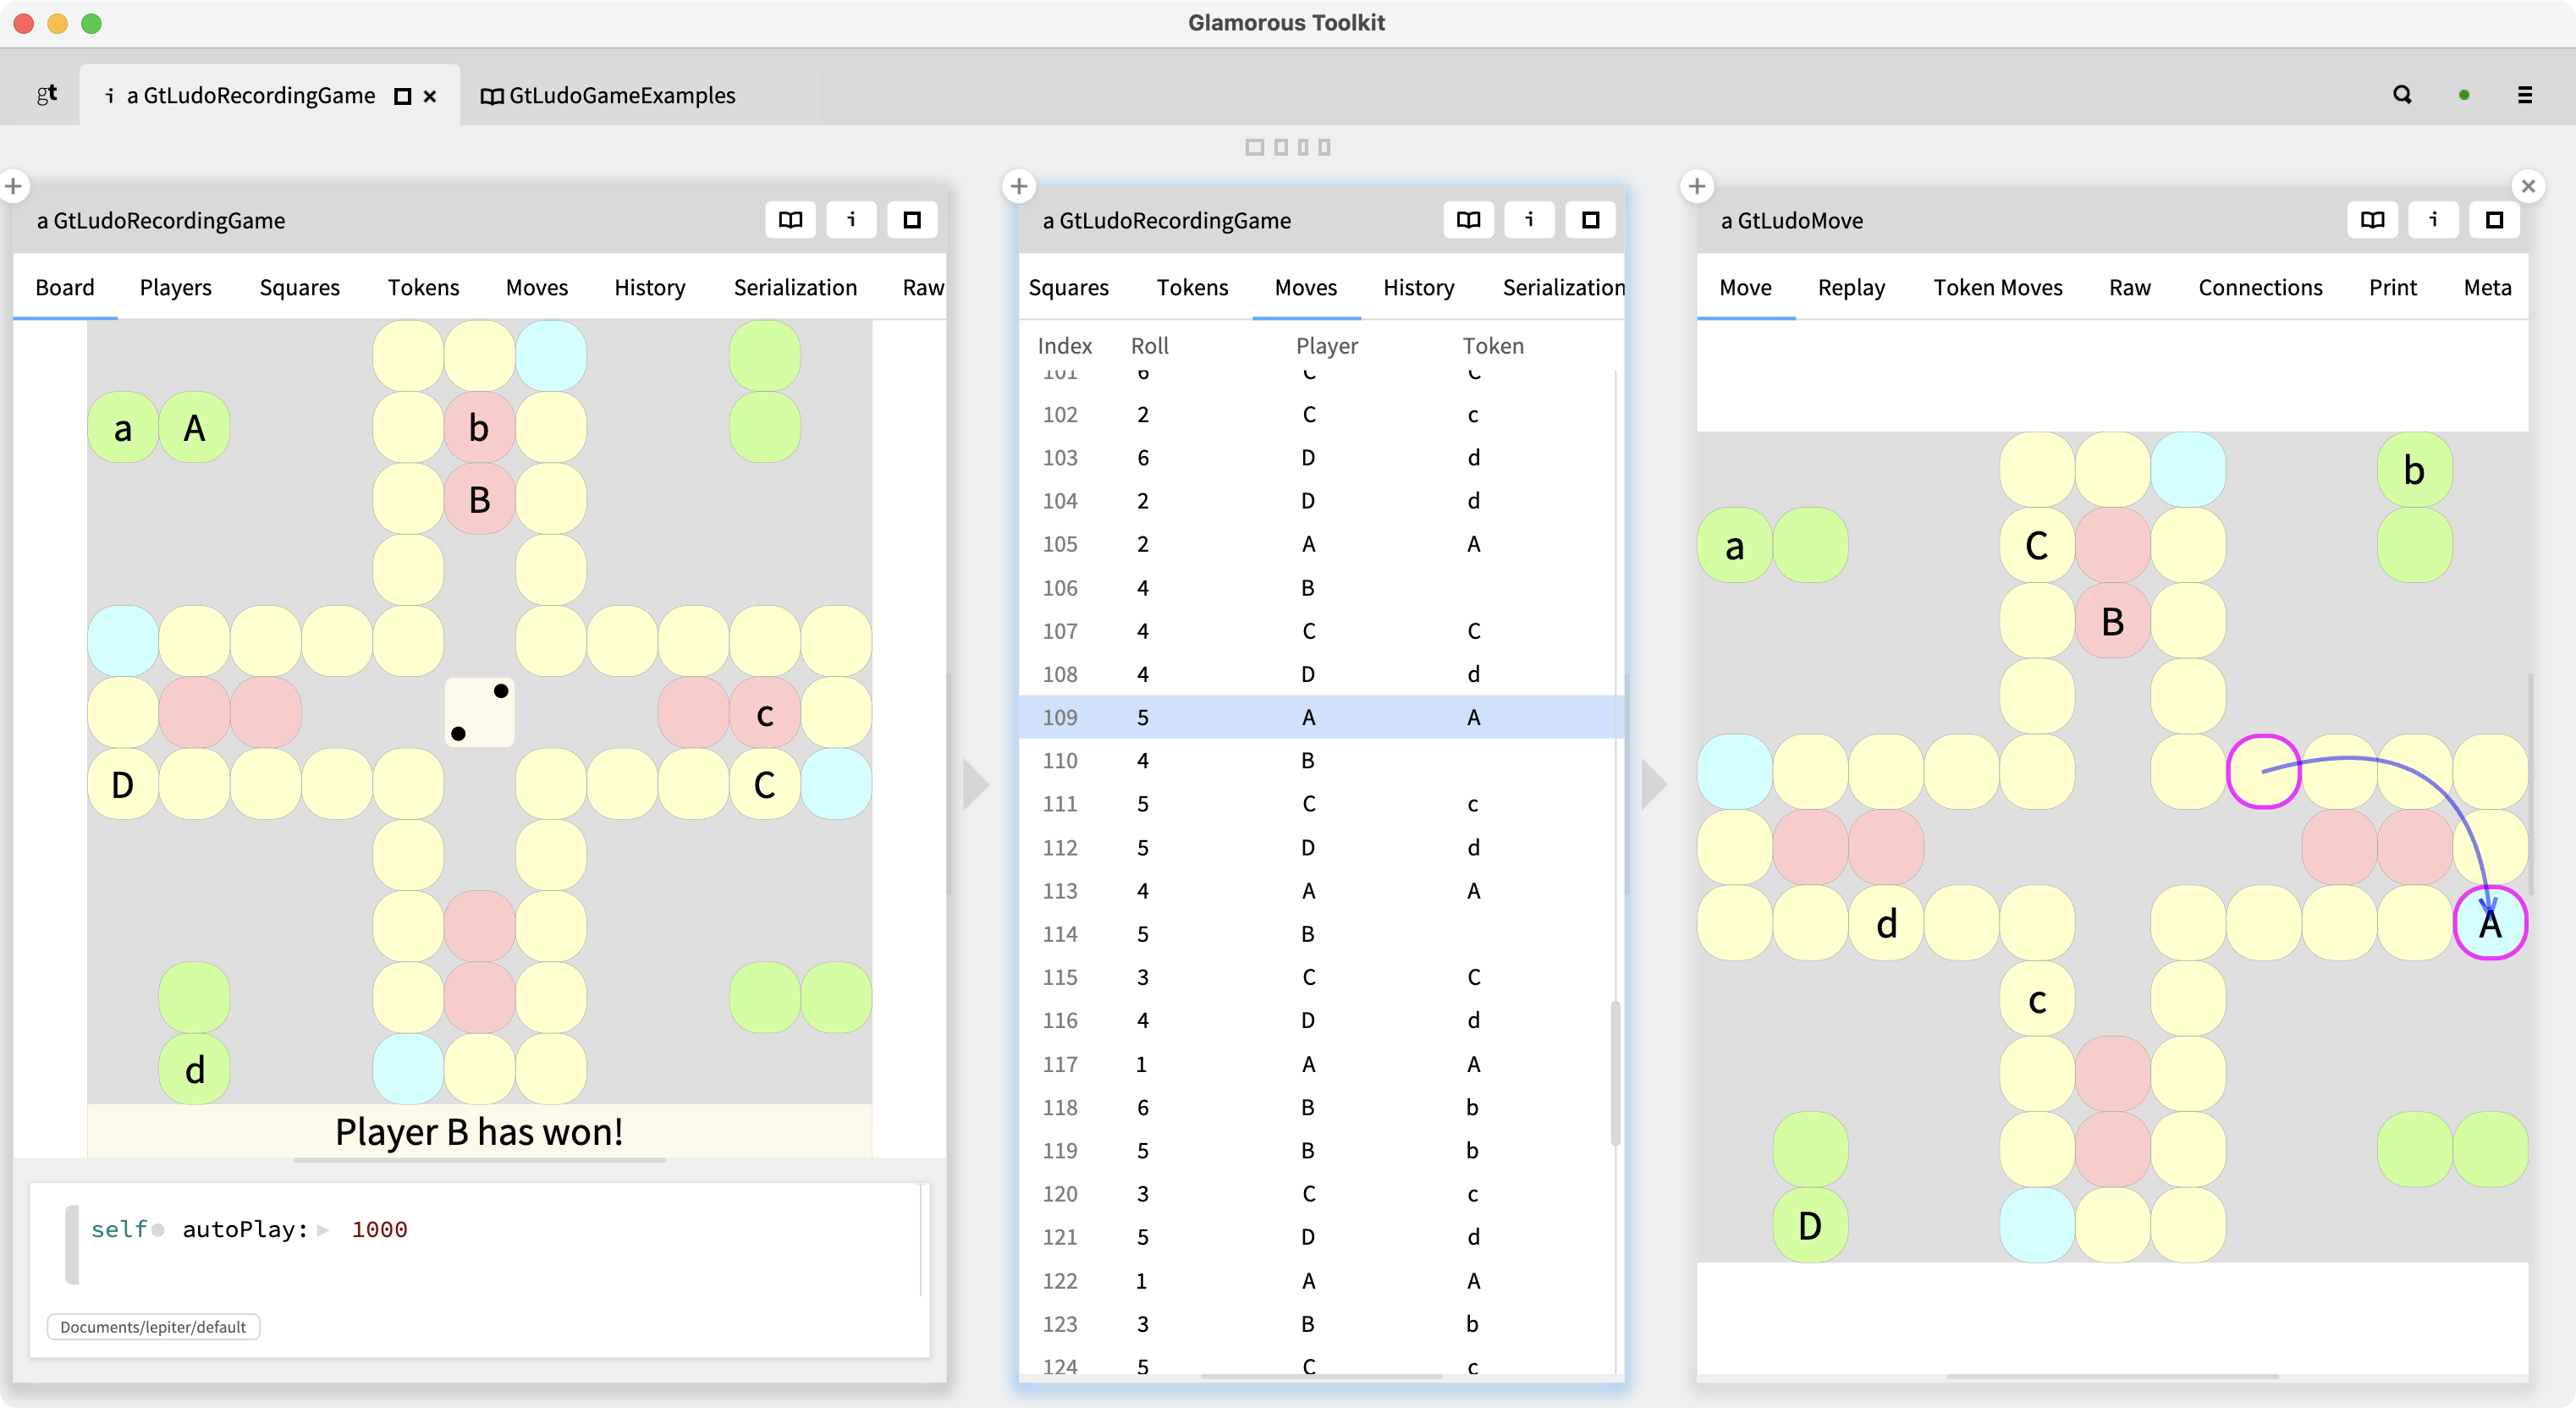
\includegraphics[width=\columnwidth]{customViews}
  \caption{Custom views of a Ludo game.}
  \label{fig:ludoViews}
\end{figure}

These views have each been created with a few lines of code, in the first and last cases leveraging the existing GUI view of the Ludo game.
The object inspector recognizes that the Ludo game object is an instance of the \lst{GtLudoRecordingGame} class, 
which has been extended with several custom views defined as annotated methods of that class.
Similarly the move object is an instance of the \st{GtLudoMove} class, which has been extended with other views specific to moves.

Two other common types of custom tools are \emph{custom actions} (\eg buttons), which perform a task and possibly spawn another tool such as an inspector, a code editor or an external web browser, and \emph{custom searches}, which query the running object model, and spawn a tool such as an object inspector on the result.

Example methods serve as both the input and output of moldable development.
Typically we start with a ``raw'', unenhanced example, such as we see in \autoref{fig:exampleCreationB}: the \st{ConcretePrice} inspector view shows just a basic ``raw'' view of the instance state of the example.
As we elaborate the examples in the EDD process, we mold them with custom tools that validate the requirements expressed by the examples.
The output of the process is then a molded example that not only checks assertions about its expected behavior, but also exposes that behavior through custom tools.

In \autoref{fig:ConcretePrice} we see another demo version of our \lst{ConcretePrice} class called \st{GtDConcretePrice}.
It has a custom view called \emph{Overview} (left pane) showing that the price is just a fixed amount of money.
In the right pane we see the code that implements this custom view.
The details of the implementation are not important here, but please note that this method consists of just a dozen lines or so of boilerplate code.
Most custom views in GT are short, and the average size of these methods is about a dozen lines.

\begin{figure}[h]
  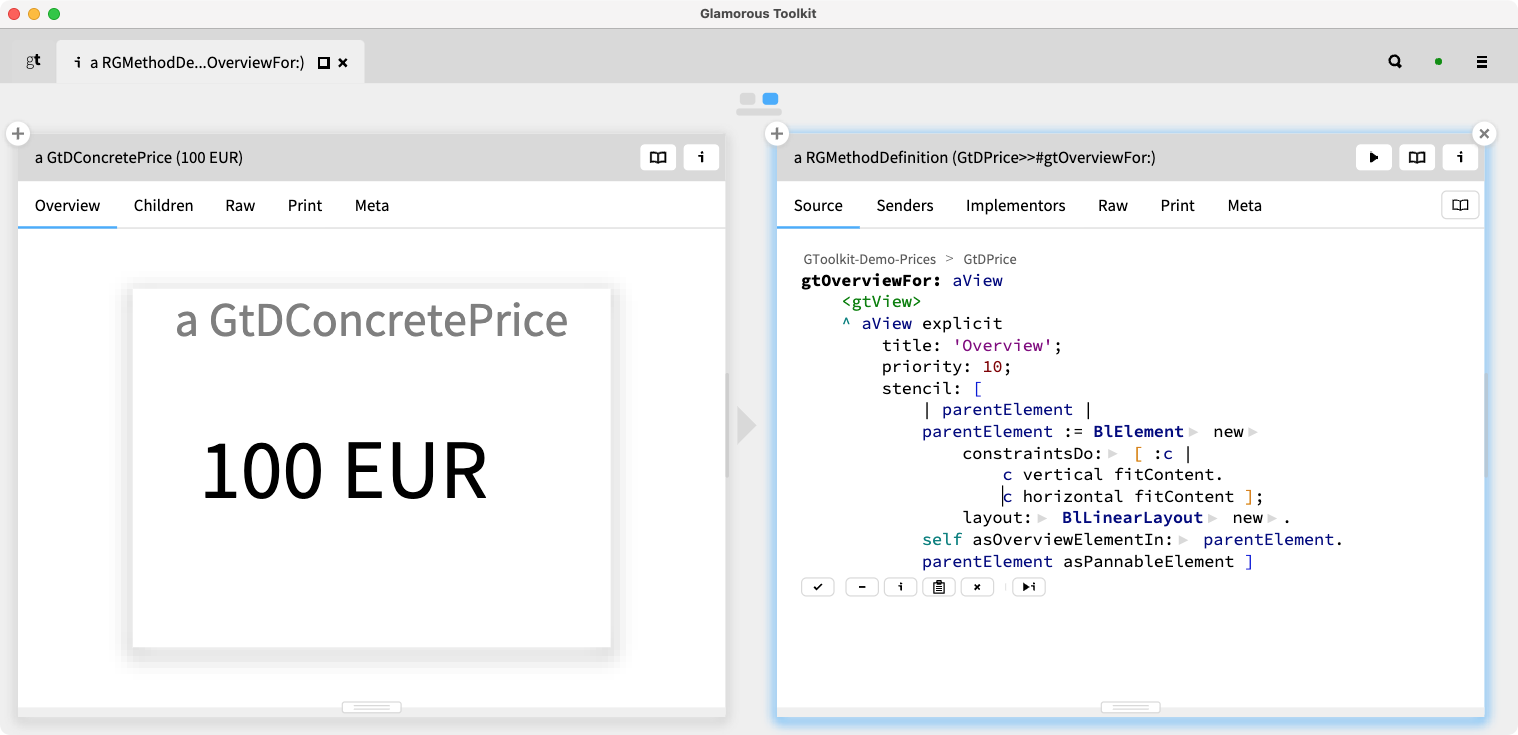
\includegraphics[width=\columnwidth]{md1-ConcretePrice}
  \caption{A ConcretePrice object with a custom view.}
  \label{fig:ConcretePrice}
\end{figure}

In \autoref{fig:DiscountedPrice} we see a more complex example of a price that has been discounted twice, first by a fixed amount, and then by a percentage.
In this case, the \emph{Overview} explains how the price has been calculated as a composition of discounts.

\begin{figure}[h]
  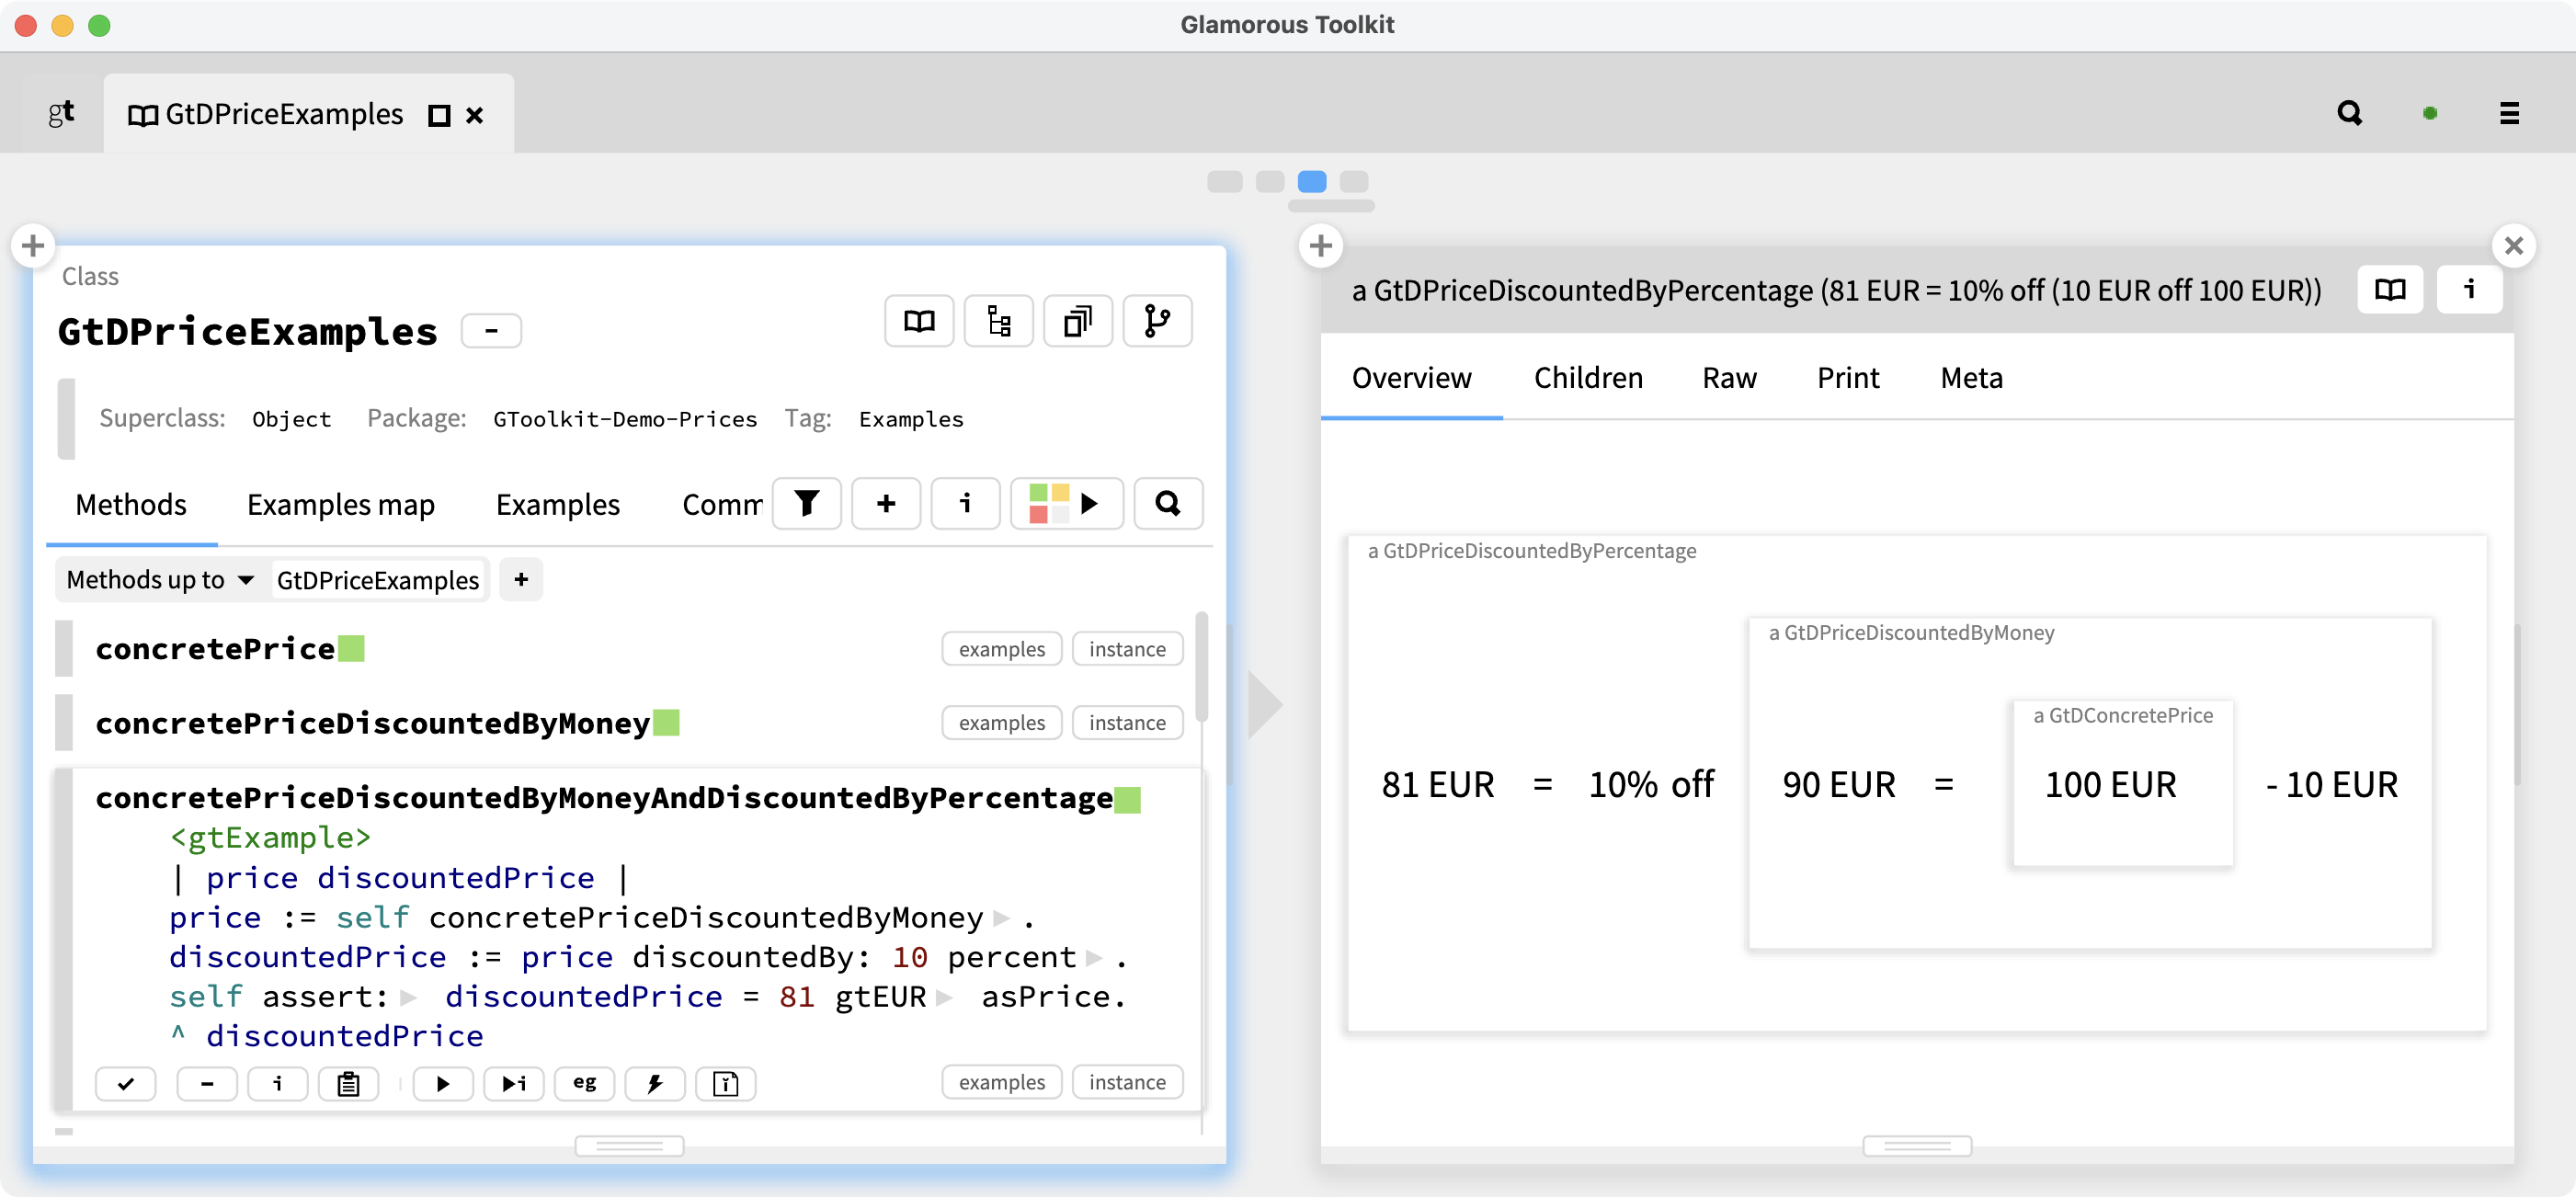
\includegraphics[width=\columnwidth]{md2-DiscountedPrice}
  \caption{A DiscountedPrice showing how it is composed.}
  \label{fig:DiscountedPrice}
\end{figure}

% ============================================================
\section{Explainable Systems using Examples}\label{sec:explainable}

\rC{A similar comment (as about the price examples not being compelling) could be made about explainability. Making software more explainable is a big deal, but the very high-level way in which you presented the examples in Section 4 failed to convince me. Not because your examples weren't interesting, but because you didn't go into enough detail for me to be able to tell whether or not you did a good job of making the code explainable. One way to address this problem might be to spend most of the paper going deep into a single, really compelling example (this could be your running example throughout the paper), instead of going for quantity.
The "tiny analysis tools" (or views?) on the examples that are accessible via tabs in your inspector-like UI are a key part of the EDD experience. Presumably you could use EDD to program them, too. Showing what that experience is like would help paint a more complete picture of what it's like to live inside your system.
In summary, I suspect there are some really good and interesting ideas here, but the paper doesn't doesn't do a great job of showing them off, or even make it clear what your contributions are.}

%\todo{Add something about creating narratives -- the custom views allow you to create both fixed narratives as notebook pages, and dynamic narratives by navigating to new views}

%\ac{Feels like we should show also a page describing prices}

Perhaps the most compelling use of examples is within live documentation.
GT includes support for knowledge bases consisting of linked notebook pages that are composed of various kinds of snippets: formatted text, images, code in various programming languages, and live examples.
An example snippet identifies an example method to be evaluated, and a view to be rendered when the notebook page is loaded.

This simple feature enables the creation of various kinds of live documentation, such as live project diaries, interactive tutorials, and live API documentation.

Let's see a few examples from the GT book, the knowledge base that comes bundled with the GT download.

In \autoref{fig:LudoBook} we see an extract of a page describing the Ludo game.
This section of the page describes the rules of the game for a new, live, embedded example of the initial move of a player.
What we see is a custom view of a move object produced by the \st{moveInitial} example method of the \st{GtLudoRecordingGameExamples} class.

\begin{figure}[h]
  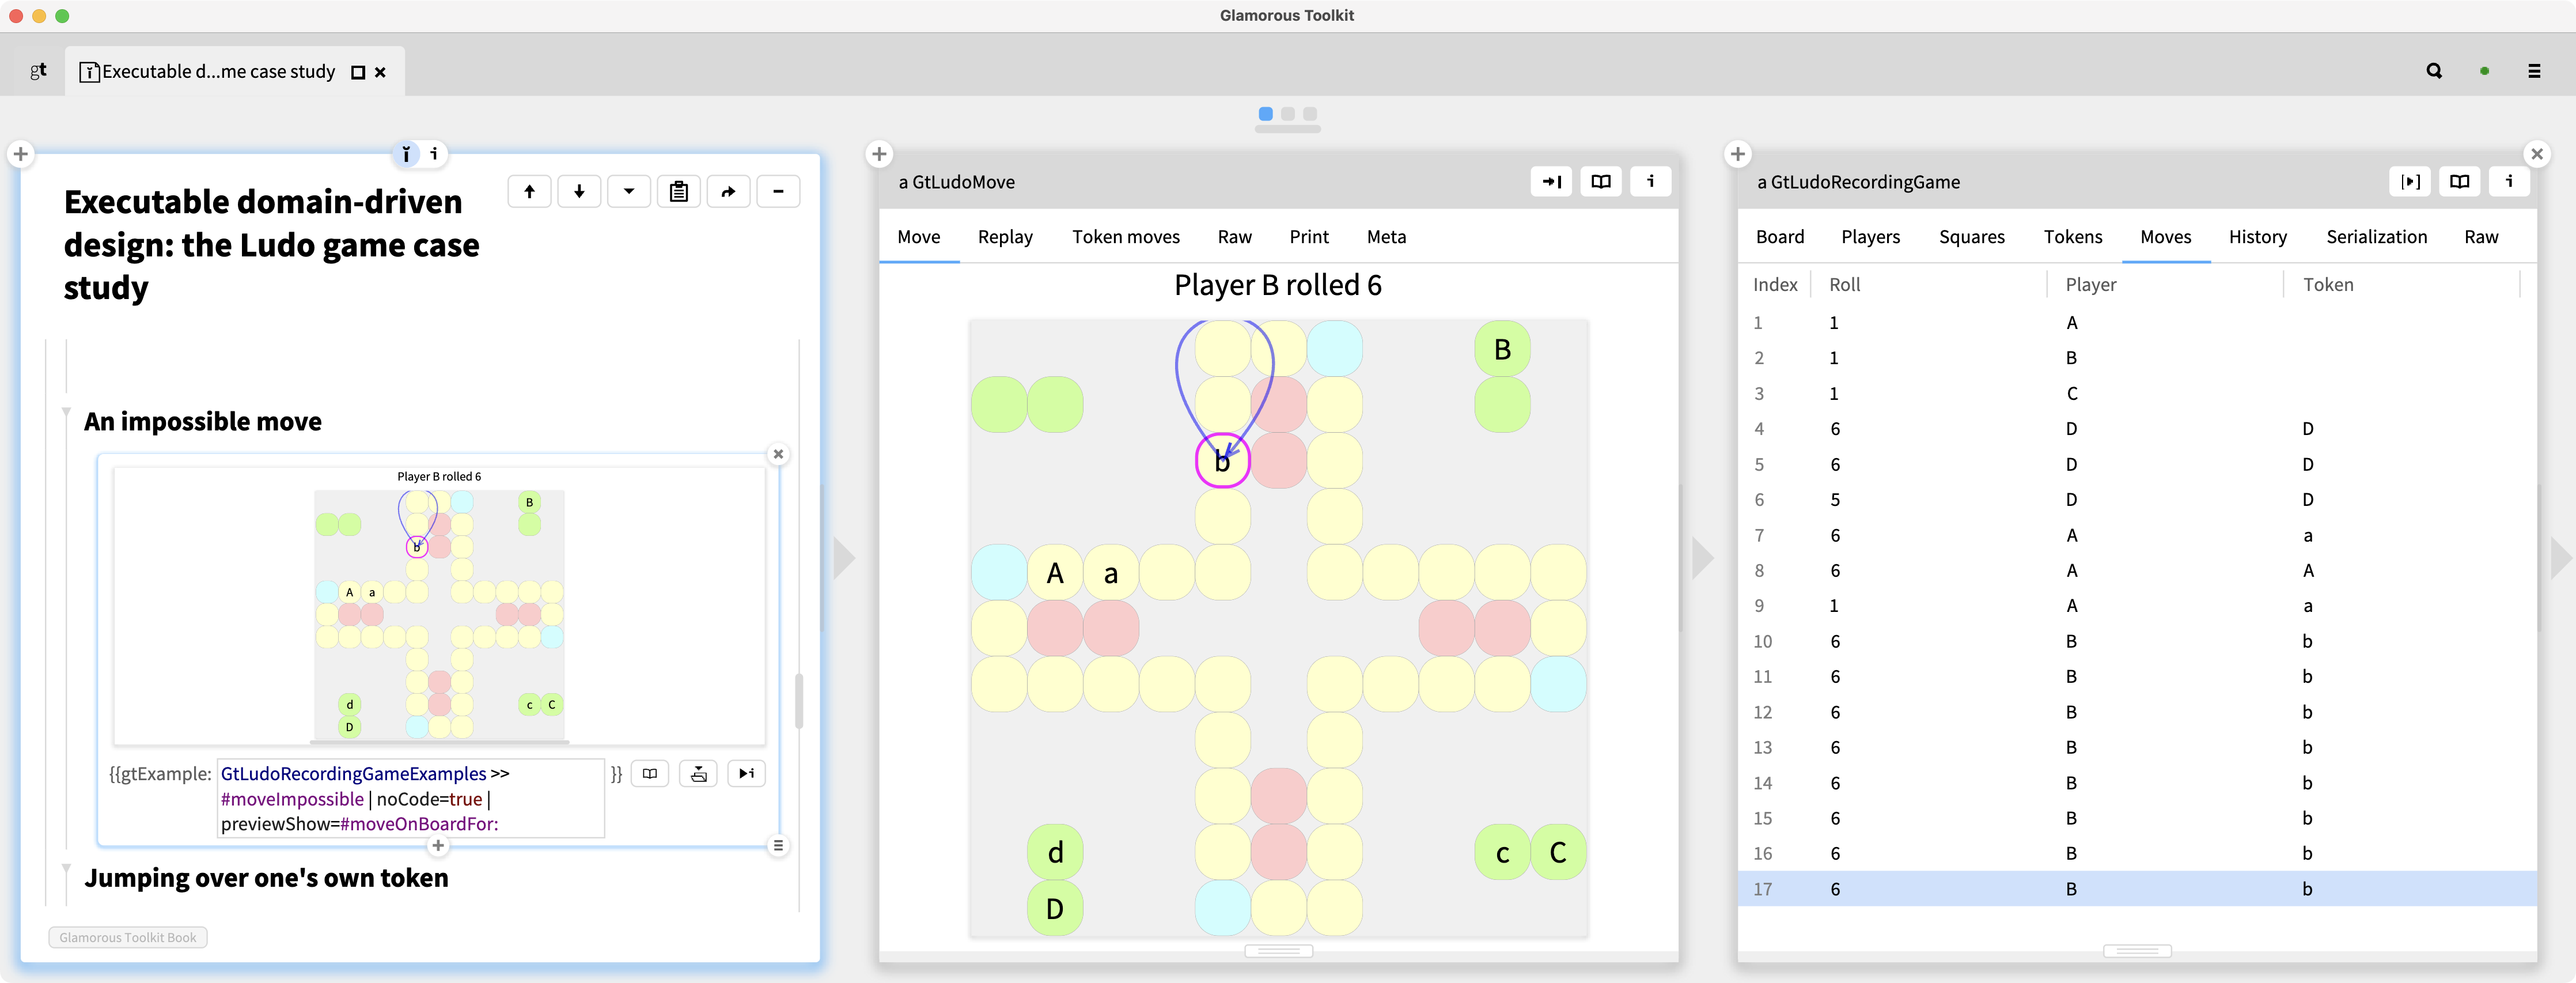
\includegraphics[width=\columnwidth]{book1-ludo-move}
  \caption{A ``Ludo'' documentation.}
  \label{fig:LudoBook}
\end{figure}

Examples can also be used effectively to explain algorithms.
In \autoref{fig:Treemap} we see a notebook page that explains how a squarified TreeMap layout algorithm works with the help of live examples.
The embedded example not only shows the final layout (left), but by diving into it (right), we can see the decision steps taken to periodically switch orientation between horizontal and vertical tree map nodes to maintain a ``squarified'' appearance.

\begin{figure}[h]
  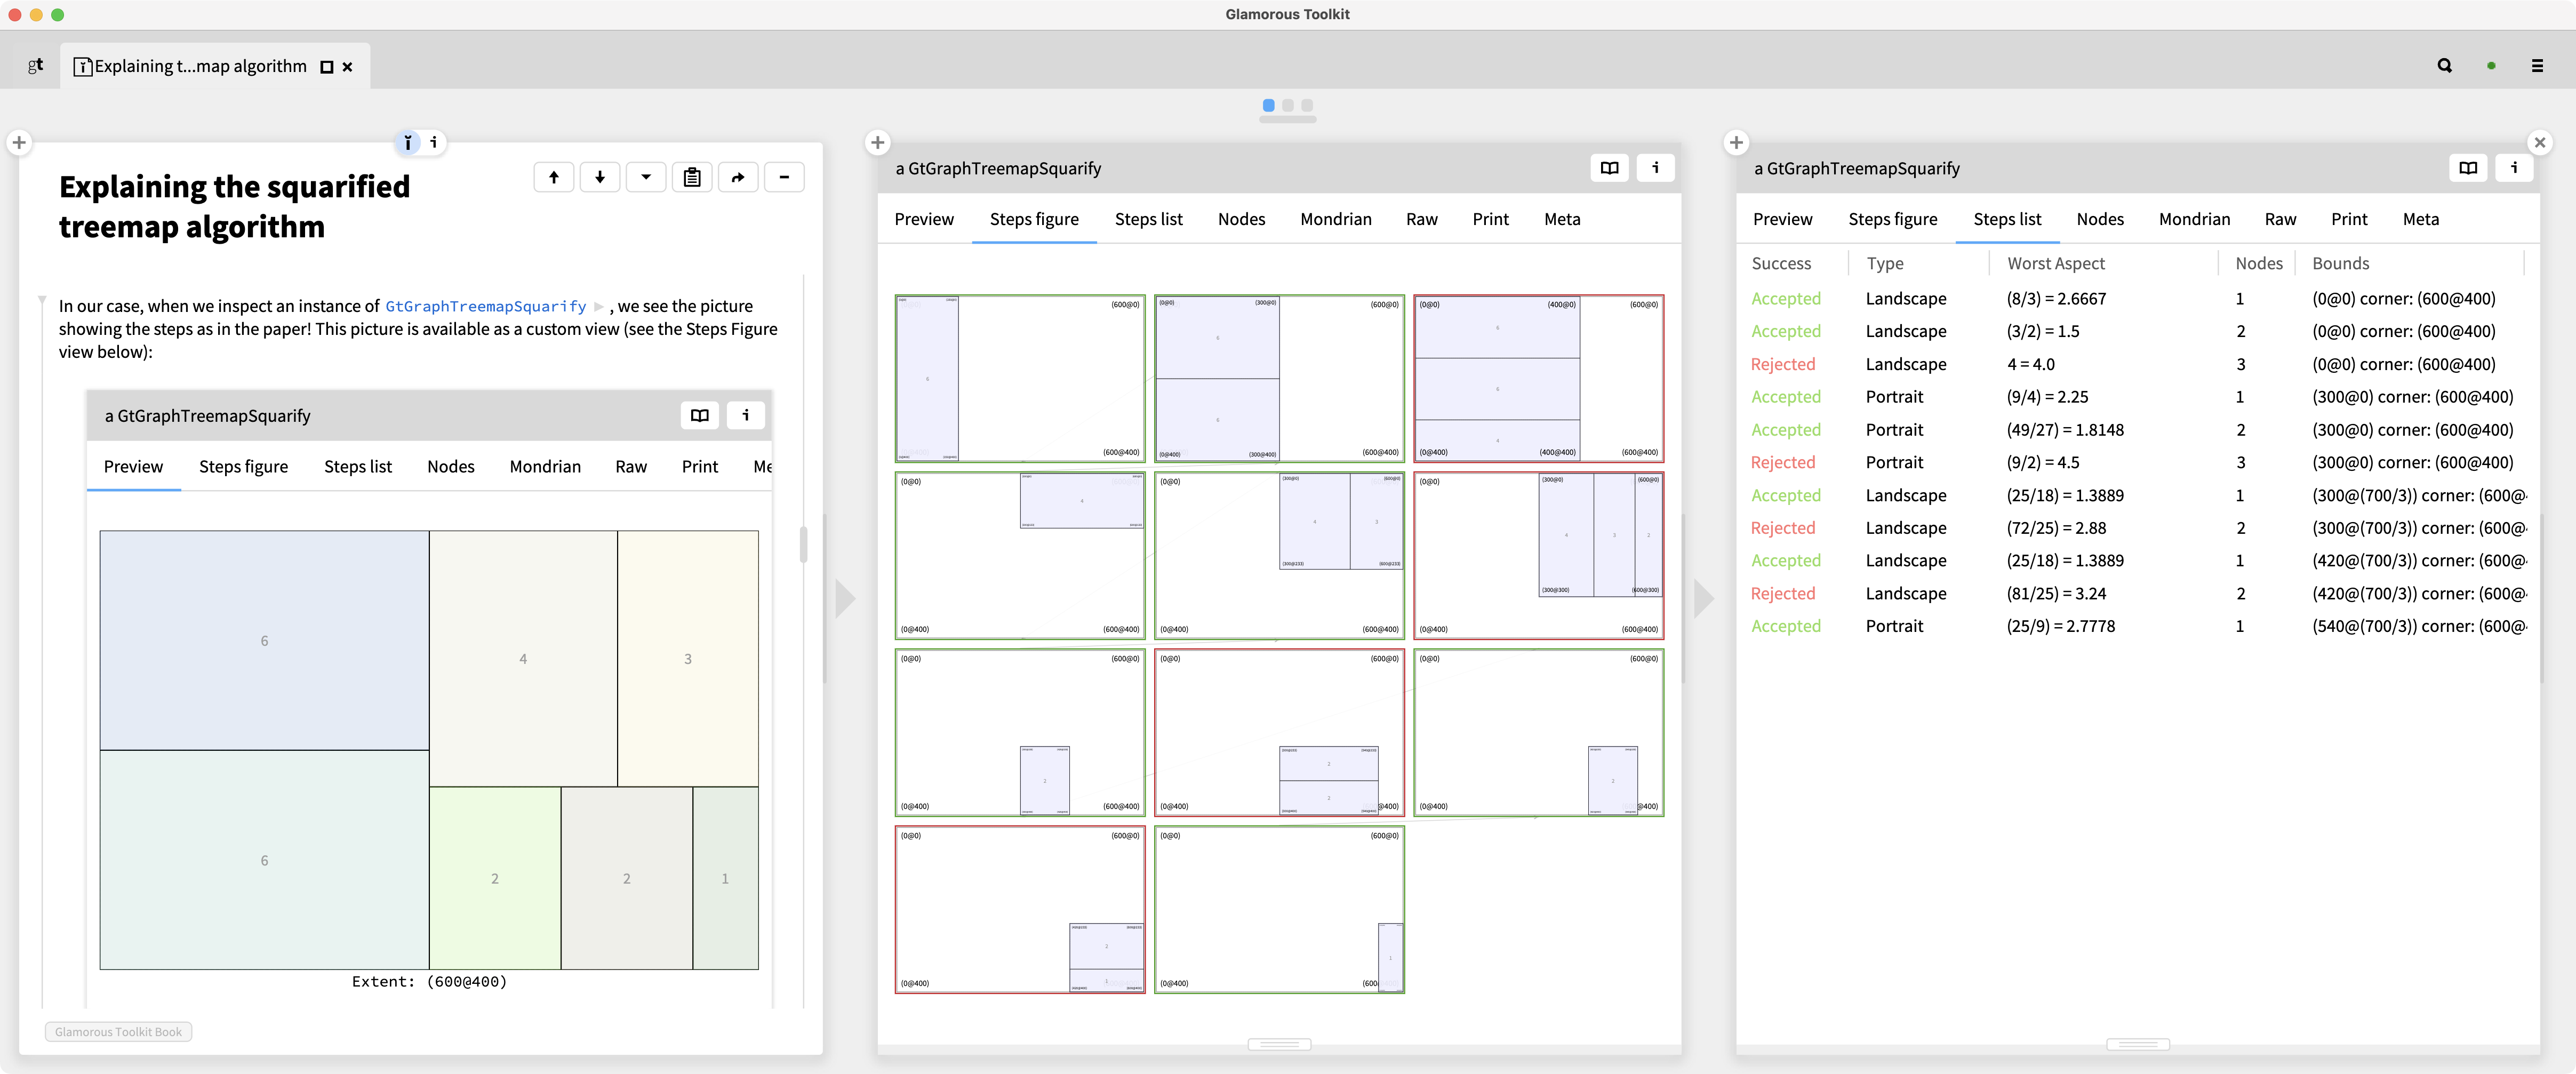
\includegraphics[width=\columnwidth]{book3-Treemap}
  \caption{Explaining a squarified TreeMap algorithm.}
  \label{fig:Treemap}
\end{figure}

Finally, \autoref{fig:Patterns} shows how examples can be used within notebook pages that explain the moldable development process itself in terms of a number of patterns~\cite{Nier24a}.
The \emph{Moldable Development patterns} page contains a live embedded map (an example) that allows you to navigate to pages describing the individual patterns.
These pages, such as \emph{Custom Search}, in turn contain other live examples to illustrate the patterns.

\begin{figure}[h]
  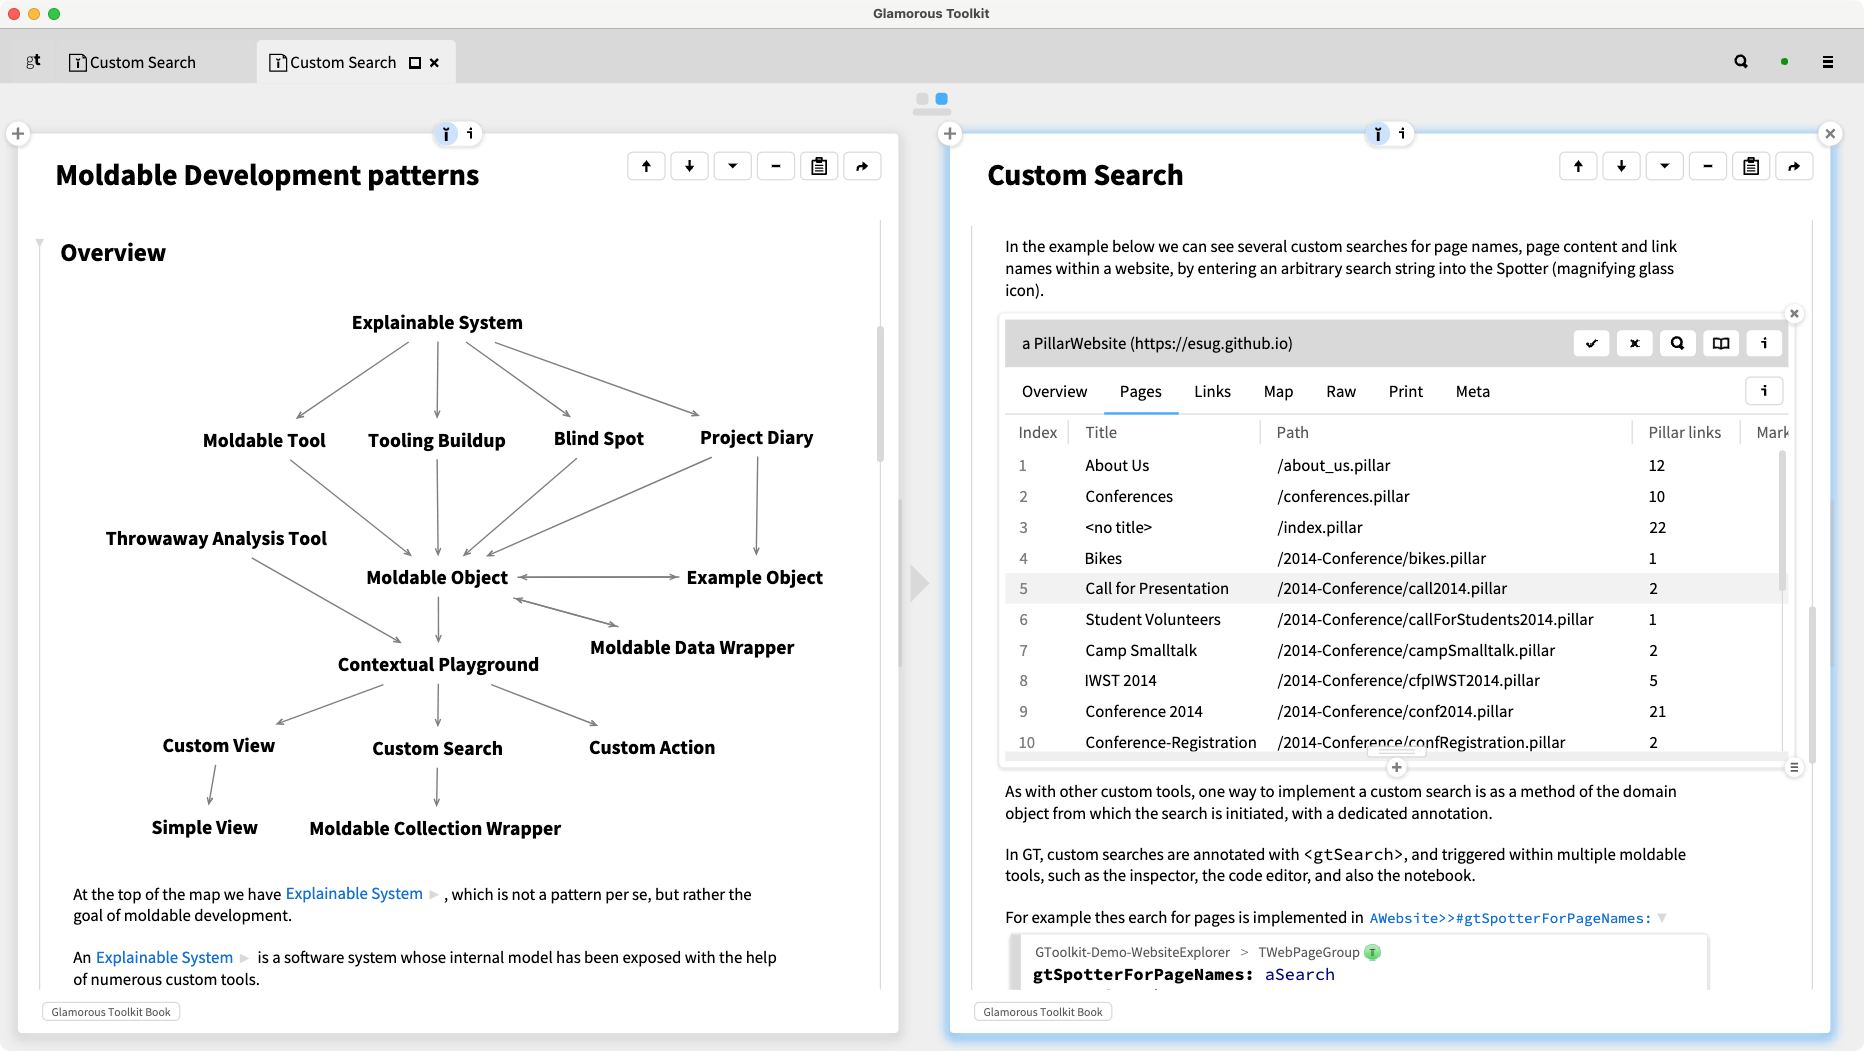
\includegraphics[width=\columnwidth]{book4-MDPatterns}
  \caption{A map of Moldable Development patterns.}
  \label{fig:Patterns}
\end{figure}

All of these illustrations show not only how example methods can be used productively to produce live documentation, but that by applying moldable development principles, the live examples can be easily enhanced with lightweight, custom tools that serve to make the examples, and the systems they are part of, truly explainable.

%\todo{Should we list statistics on examples, snippets, pages etc.?\\
%There are 10804 example methods averaging 13.068 LoC
%compared with
%24552 test methods averaging 9.58 LoC.\\
%The GT Book has 456 pages, of which 97 containing example snippets, for a total of 332 example snippets.
%Two pages have 22 examples.
%}

\rC{You explore EDD in the context of the Glamorous Toolkit. This work would be more widely applicable (thus more valuable) if you could somehow disentangle your contributions from GT. To that end, consider adding a section that outlines the set language and programming environment features that are needed in order to take full advantage of EDD and enable the flavor of live programming you talk about in the paper.}

% ============================================================
\section{Related work}\label{sec:related}
\rA{I would have liked to see some comparison between this programming workflow and a REPL-driven programming workflow, which feel quite similar in that they both support open-ended exploration and prototyping with live objects. Is the main difference that this system stores examples for later, and provides custom dev tools for inspecting and editing objects?}

\rA{A couple related ideas that you might find interesting to review and possibly cite:\\
- Example Centric Programming, Edwards OOPSLA 2004 notes the relationship between examples and tests: https://www.subtext-lang.org/OOPSLA04.pdf\\
- The Clojure [REBL data browser](https://docs.datomic.com/other-tools/REBL.html) has some related ideas around visualizing data and showing examples, described in [this video](https://www.youtube.com/watch?v=Qx0-pViyIDU)}

\rB{The paper misses one closely related work from OOPSLA 2024 (https://doi.org/10.1145/1052883.1052894) that proposed example-centric programming (and debugging). How does EDD differ from example-centric programming? Maybe they are different in some ways that I missed. The paper should include a thorough review of this work and discuss how EDD relates to example-centric programming.}


Bush was the first to dream of a computerized ``memex'' of stored knowledge~\cite{Bush45a}, through which a user could trace an associative ``trail'' of interconnected text and multimedia resources.
The memex vision inspired Engelbart's NLS~\cite{Enge68a}, the first system to demonstrate human interaction with a computer mouse, windows, and hypertext features.
Knuth first pioneered the implementation of a computational notebook, called WEB, to support ``literate programming'' through the combination of text, graphics, and live code~\cite{Knut97a}.

Modern notebook systems such as Jupyter\footnote{\url{https://jupyter.org}}, MATLAB Live Scripts\footnote{\url{https://www.mathworks.com/}} and Wolfram Notebooks\footnote{\url{https://www.wolfram.com/notebooks/}} all offer the ability to embed live instances of classes within notebook pages, but these live examples are neither integrated with unit testing frameworks, not do they support custom tooling with the help of moldable tools to tailor the user experience.

%\todo{Add something on Shri's Executable Examples paper? Wren19a}
%% https://cs.brown.edu/~sk/Publications/Papers/Published/wk-examplar/

The \emph{Test Data Builder} pattern~\cite{Free09a} introduces factory methods for test fixtures, also potentially reducing code duplication in tests, but the resulting objects are only intended as inputs for tests, not their outputs.
The resulting examples are not accessible as the output of a green test.

Cucumber~\cite{Hell17a} is a software tool that supports Behavior-Driven Development through business rules specified in the Gherkin language.
These rules include the specification of ``examples'' (AKA scenarios) that illustrate business rules.
The usage of these examples, however, is restricted to the context of the business rules, and they are not intended as the outputs of tests.

Modern testing frameworks such as pytest~\cite{Okke22a}, allow tests to be parameterized by fixtures specified as separate methods.
Here too, however, fixtures are only seen as inputs to tests, not as outputs.

% ============================================================
\section{Conclusion}\label{sec:conclusion}

Having tests be factories for examples is a small, but potentially groundbreaking enhancement.
EDD enhances TDD by making examples rather than tests be the focus of the development process.
By enhancing examples with lightweight, custom tools, they help users answer all kinds of analysis questions.
By embedding examples in live documentation, they make software systems explainable.
As a consequence, up-to-date documentation becomes merely a side-effect of applying EDD.

%\begin{acks}
%\end{acks}

% ============================================================

\bibliographystyle{ACM-Reference-Format}
\bibliography{eddBridge}

\end{document}
\endinput

% ============================================================

\begin{inparaenum}[(i)]
	\item 
\end{inparaenum}

\begin{figure}[h]
  \includegraphics[width=\columnwidth]{xxx}
  \caption{xxx.}
  \label{fig:xxx}
\end{figure}

